\documentclass{report}
\usepackage[T1]{fontenc} % Fontes T1
\usepackage[utf8]{inputenc} % Input UTF8
\usepackage[backend=biber, style=ieee]{biblatex} % para usar bibliografia
\usepackage{csquotes}
\usepackage[portuguese]{babel} %Usar língua portuguesa
\usepackage{blindtext} % Gerar texto automaticamente
\usepackage[printonlyused]{acronym}
\usepackage{hyperref} % para autoref
\usepackage{graphicx}
\usepackage{indentfirst}
\usepackage{float}
\usepackage{subcaption}
\usepackage{makecell}


\bibliography{bibliografia}


\begin{document}
%%
% Definições
%
\def\titulo{VIDA MARINHA}
\def\data{DATA}
\def\autores{Carolina Sousa Teixeira, João Diogo da Silva Correia Teixeira Martins}
\def\autorescontactos{(115903) carolinasteixeira@ua.pt, (120284) joaodiogomartins@ua.pt}
\def\versao{VERSAO 1}
\def\departamento{Dept. de Eletrónica, Telecomunicações e Informática}
\def\empresa{Universidade de Aveiro}
\def\logotipo{ua.pdf}
%
%%%%%% CAPA %%%%%%
%
\begin{titlepage}

\begin{center}
%
\vspace*{50mm}
%
{\Huge \titulo}\\ 
%
\vspace{10mm}
%
{\Large \empresa}\\
%
\vspace{10mm}
%
{\LARGE \autores}\\ 
%
\vspace{30mm}
%
\begin{figure}[h]
\center
\includegraphics{\logotipo}
\end{figure}
%
\vspace{30mm}
\end{center}
%
\begin{flushright}
\versao
\end{flushright}
\end{titlepage}

%%  Página de Título %%
\title{%
{\Huge\textbf{\titulo}}\\
{\Large \departamento\\ \empresa}
}
%
\author{%
    \autores \\
    \autorescontactos
}
%
\date{\today}
%
\maketitle

\pagenumbering{roman}

%%%%%% RESUMO %%%%%%  200-300 palavras
\begin{abstract}

Os oceanos acolhem uma imensa diversidade de espécies desde mamíferos até invertebrados, passando até por organismos fotoautotróficos e decompositores, as quais vivem em ecossistemas diversificados, tanto pelas características das suas águas como pela profundidade a que se situam, garantindo aos mares uma abundância de seres, vivos e não vivos, com imensas características e interações variadas ainda por explorar. 

Infelizmente muitas destas maravilhas marinhas encontram-se em perigo face às mudanças ambientais e ações antrópicas, que poluem e magoam os ecossistemas e os seus habitantes levando até à extinção de algumas espécies, e por isso é necessário consciencializar a população e agir de forma a cancelar o efeito destas ameaças e restaurar os ambientes marinhos.

Este relatório tem como propósito informar o leitor sobre a complexidade das àguas marinhas, destacando os seus principais ecossistemas e descrevendo as mudanças observáveis de acordo com a profundidade, assim como a diversidade dos seres vivos, a sua classificação, diferenças fisiológicas e como eles se relacionam entre si, bem como o valor de cada um destes aspetos e descrevendo vários perigos que eles enfrentam face às ameaças ambientais do seu dia-a-dia, juntamente com possíveis soluções para estes problemas, desde medidas mais indiretas como a consciencialização das populações até medidas concretas como a criação de áreas marinhas protegidas.

\end{abstract}

%%%%%% Agradecimentos %%%%%%
% Segundo glisc deveria aparecer após conclusão...
%\renewcommand{\abstractname}{Agradecimentos}
%\begin{abstract}
%Eventuais agradecimentos.
%Comentar bloco caso não existam agradecimentos a fazer.
%\end{abstract}

\renewcommand{\contentsname}{Índice}
\tableofcontents
% \listoftables     % descomentar se necessário
% \listoffigures    % descomentar se necessário


%%%%%%%%%%%%%%%%%%%%%%%%%%%%%%%
\clearpage
\pagenumbering{arabic}

%%%%%%%%%%%%%%%%%%%%%%%%%%%%%%%%
\chapter{Introdução}
\label{chap.introducao}
Os mares apresentam uma enorme diversidade de animais, plantas, organismos e microrganismos, assim como de ecossistemas e habitats onde estes organismos vivem. Existe uma grande variação fenotípica e genotípica em seres vivos dependo das águas e de quão profundo estes se encontram. É por causa desta abundância de organismos e interações que a vida marinha apresenta um papel tão importante na natureza do planeta e deve ser protegida face à influência dos comportamentos humanos influentes na mudança climática, tendo sido essa a principal razão por detrás da escolha deste tema.

O documento divide-se em 4 capítulos, no \autoref{chap.classificação} é tratada a biologia marinha e classificação dos organismos marinhos tais como os peixes, mamíferos aquáticos, invertebrados e algas, assim como as interações simbióticas entra os diferentes organismos. No \autoref{chap.biodiversidade} são descritos os vários ecossistemas e as espécies específicas de habitats encontrados em cada sistema, assim como a biodiversidade de diferentes seres vivos dependendo da profundidade onde são encontrados. Já no \autoref{chap.impactos} são descritas mudanças observadas na vida marinha face às alterações climáticas e ações humanas como a pesca excessiva e também medidas de conservação a serem tomadas devido a estes problemas.

\chapter{Classificação da Vida Marinha}
\label{chap.classificação}

\section{Peixes}
Os peixes, como grupo de vertebrados marinhos, podem ser classificados em duas categorias: Peixes Ósseos (\textit{Osteichtyes}) e Peixes Cartilaginosos (\textit{Chondrichthyes}). Neste contexto, exploraremos as diferenças entre estes dois grupos de peixes, destacando as suas características únicas e contribuições para o ambiente marinho. 
\subsection{Peixes Ósseos (\textit{Osteichtyes})}
\subsubsection{Anatomia e Morfologia}
Os peixes ósseos, pertencentes à classe \textit{Osteichtyes}, exibem uma variedade impressionante de características anatómicas e morfológicas que são essenciais para a sua adaptação ao ambiente aquático. Estas características contribuem para a eficiência na natação, captura de alimentos, respiração e equilíbrio hidrodinâmico:
\begin{itemize}
	\item \textbf{Esqueleto ósseo}: O esqueleto dos peixes ósseos é predominantemente composto por tecidos ósseos, que lhes confere uma estrutura robusta e flexível. A coluna vertebral confere suporte e flexibilidade para movimentos ágeis, enquanto o crânio protege os órgãos vitais, como o cérebro e os órgãos sensoriais. Costelas e espinhos ósseos reforçam a estrutura do corpo, contribuindo para a proteção dos órgãos internos.
\\
\\
\\
\\
	\item \textbf{Barbatanas}: As barbatanas dos peixes ósseos desempenham um papel crucial na sua locomoção e estabilidade na água. A barbatana dorsal, situada no dorso, auxilia na estabilidade lateral, enquanto as nadadeiras peitorais e pélvicas, posicionadas nos lados do corpo, são fundamentais para a direção e equilíbrio durante a natação. A barbatana anal, localizada na parte inferior do corpo, trabalha em conjunto com a barbatana dorsal para controlar a posição vertical do peixe.
	
	\item \textbf{Escamas}: A presença de escamas oferece proteção contra predadores e minimiza a resistência ao deslocamento na água. Existem dois tipos principais de escamas em peixes ósseos: as ciclóides, redondas e lisas, e as ctenóides, com bordas dentadas e uma textura áspera.
	
	\item \textbf{Boca e Mandíbulas}: A estrutura da boca e das mandíbulas varia de acordo com a dieta de cada espécie. As mandíbulas são equipadas com dentes adaptados à alimentação, sendo afiados em predadores e adequado para trituração em herbívoros.
	
	\item \textbf{Guelras e Opérculo}: As guelras, localizadas nas laterais da cabeça, são responsáveis pela absorção de oxigénio da água e pela eliminação de dióxido de carbono. Protegendo as guelras, encontramos o óperculo, uma cobertura óssea que contribui para a proteção dessas estruturas vitais.
\end{itemize}


\subsubsection{Classificação Taxonomica}
\begin{enumerate}
	\item \textbf{Ordem: Salmoniformes}
	\begin{itemize}
		\item \textbf{Família: Salmonidae}
		
Os peixes da família Salmonidae, como por exemplo o Salmão-do-Atlântico (\textit{Salmo salar}) (\ref{fig:salmao}), e a Truta-arco-íris (\textit{Oncorhynchus mykiss}) (\ref{fig:truta}), são conhecidos pela sua migração anádroma, ou seja, eles passam parte da sua vida no oceano e retornam aos rios para se reproduzirem.
	\end{itemize}
	
	\begin{figure}[H]
	\center
    		\begin{subfigure}{.5\textwidth}
    		\center
        		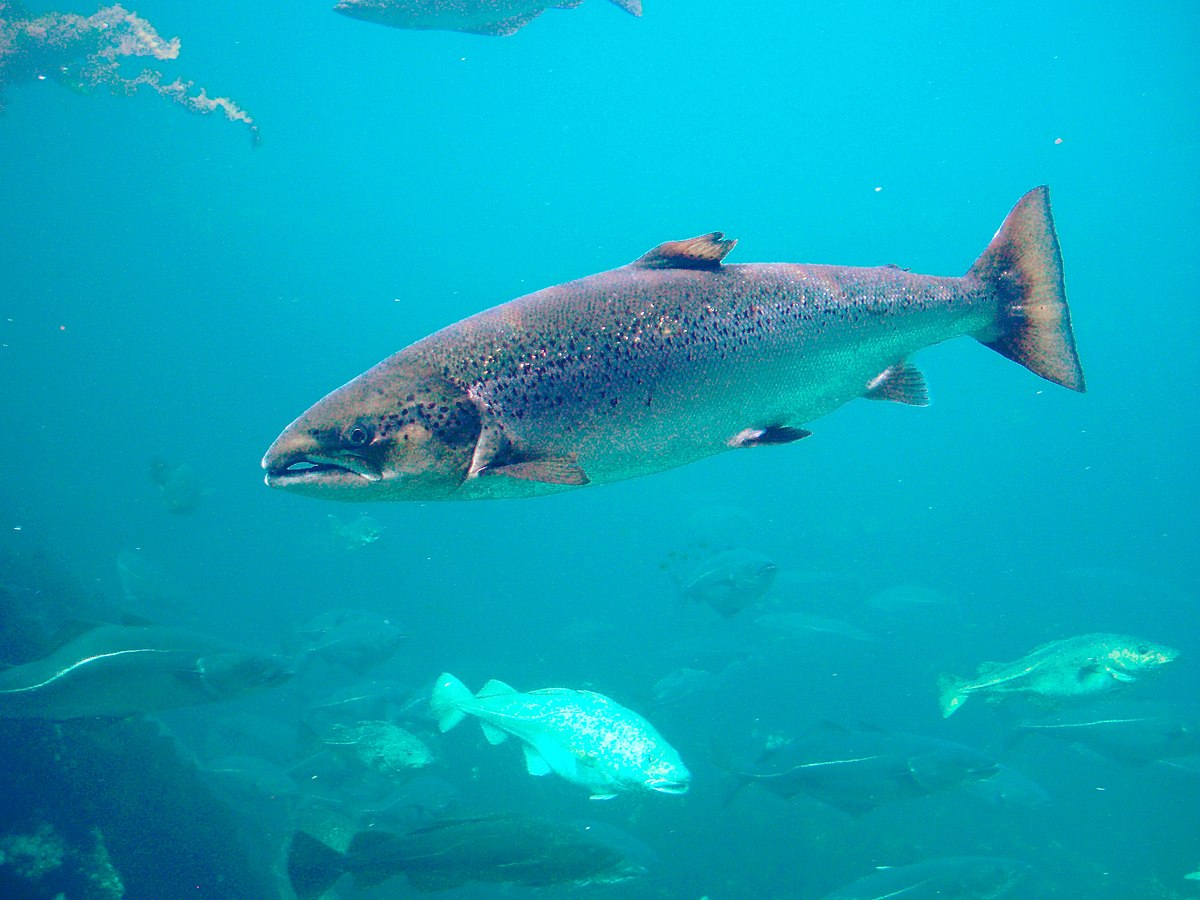
\includegraphics[height=4cm]{imagens/salmao.jpg}
        		\caption{\textit{Salmo salar}}
        		\label{fig:salmao}
    		\end{subfigure}%
   		\begin{subfigure}{.5\textwidth}
    		\center
        		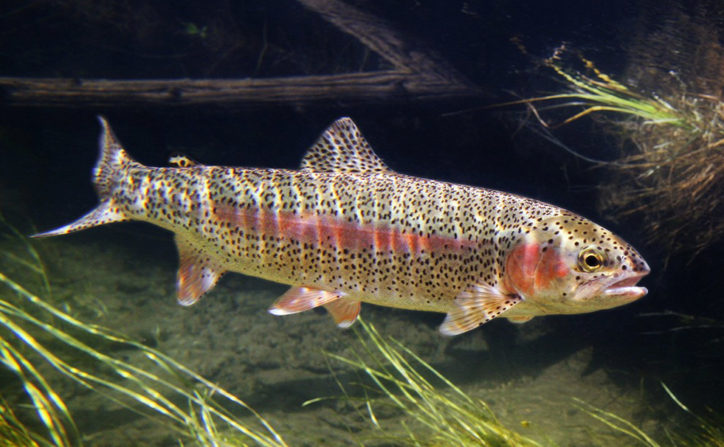
\includegraphics[height=4cm]{imagens/truta.jpg}
        		\caption{\textit{Oncorhynchus mykiss}}
       	 	\label{fig:truta}
    		\end{subfigure}
    		\caption{Familia Salmonidae}
    		\label{fig:salmonidae}
	\end{figure}
	
	
	
	\item \textbf{Ordem: Perciformes}
	\begin{itemize}
		\item \textbf{Família: Pomacentridae}

Os Peixes-palhaço (\textit{Amphiprionidae}) (\ref{fig:peixepalhaço}) da família Pomacentridae são conhecidos pela sua relação simbiótica com as anémonas-do-mar. São pequenos, coloridos porém agressivos na proteção do seu território.
	\end{itemize}
		
	\begin{figure}[H]
	\center
        	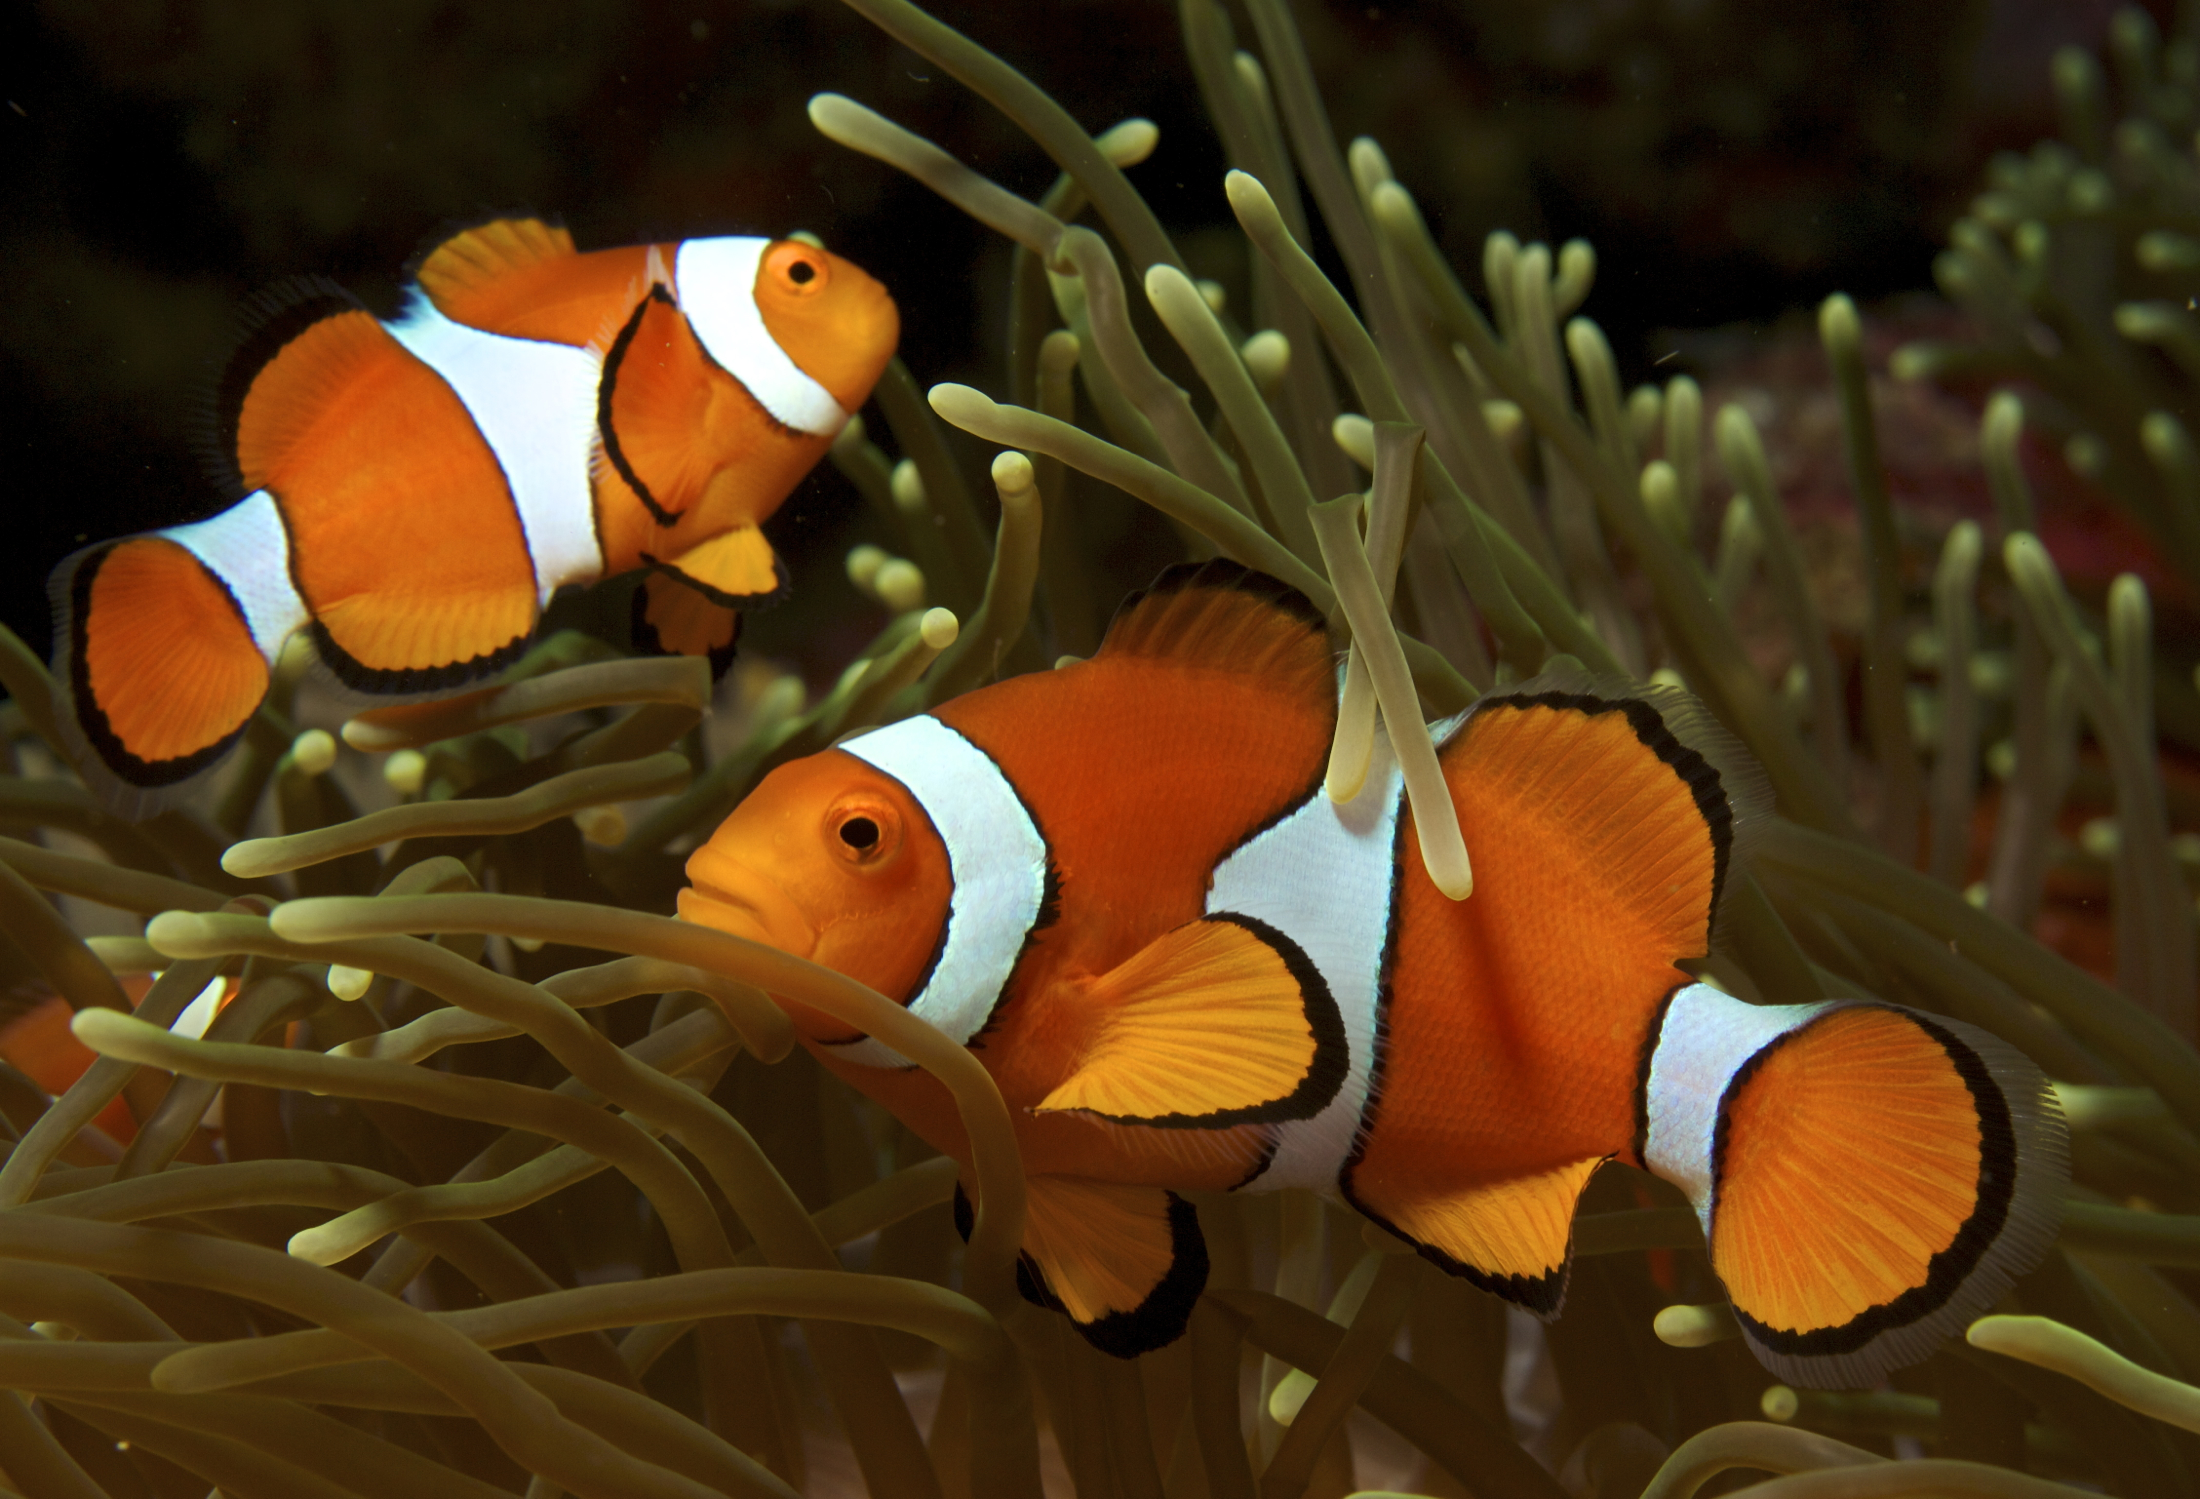
\includegraphics[height=4cm]{imagens/peixepalhaco.jpg}
        	\caption{\textit{Amphiprionidae}}
        	\label{fig:peixepalhaço}
	\end{figure}
		
	
	
	\item \textbf{Ordem: Cypriniformes}
	\begin{itemize}
		\item \textbf{Família: Cyprinidae}

Os peixes da família Cyprinidae, como a Carpa Comum (\textit{Cyprinus carpio}) (\ref{fig:carpa}) e o Barbo-d'água-doce (\textit{Barbus barbus}) (\ref{fig:barbo}), são predominantemente de água doce, possuem um corpo alongado e barbos, estruturas sensoriais nas mandíbulas.
	\end{itemize}
	
	\begin{figure}[H]
	\center
    		\begin{subfigure}{.5\textwidth}
    		\center
        		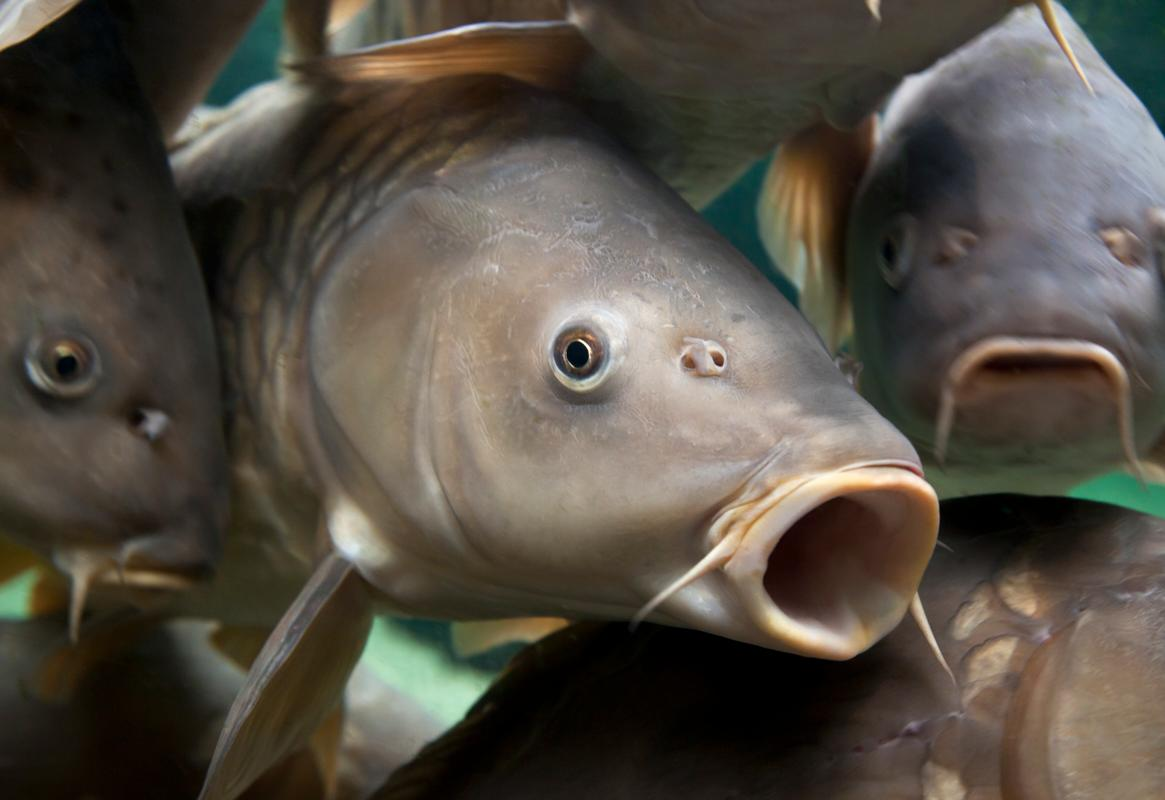
\includegraphics[height=4cm]{imagens/carpa.jpg}
        		\caption{\textit{Cyprinus carpio}}
        		\label{fig:carpa}
    		\end{subfigure}%
   		\begin{subfigure}{.5\textwidth}
    		\center
        		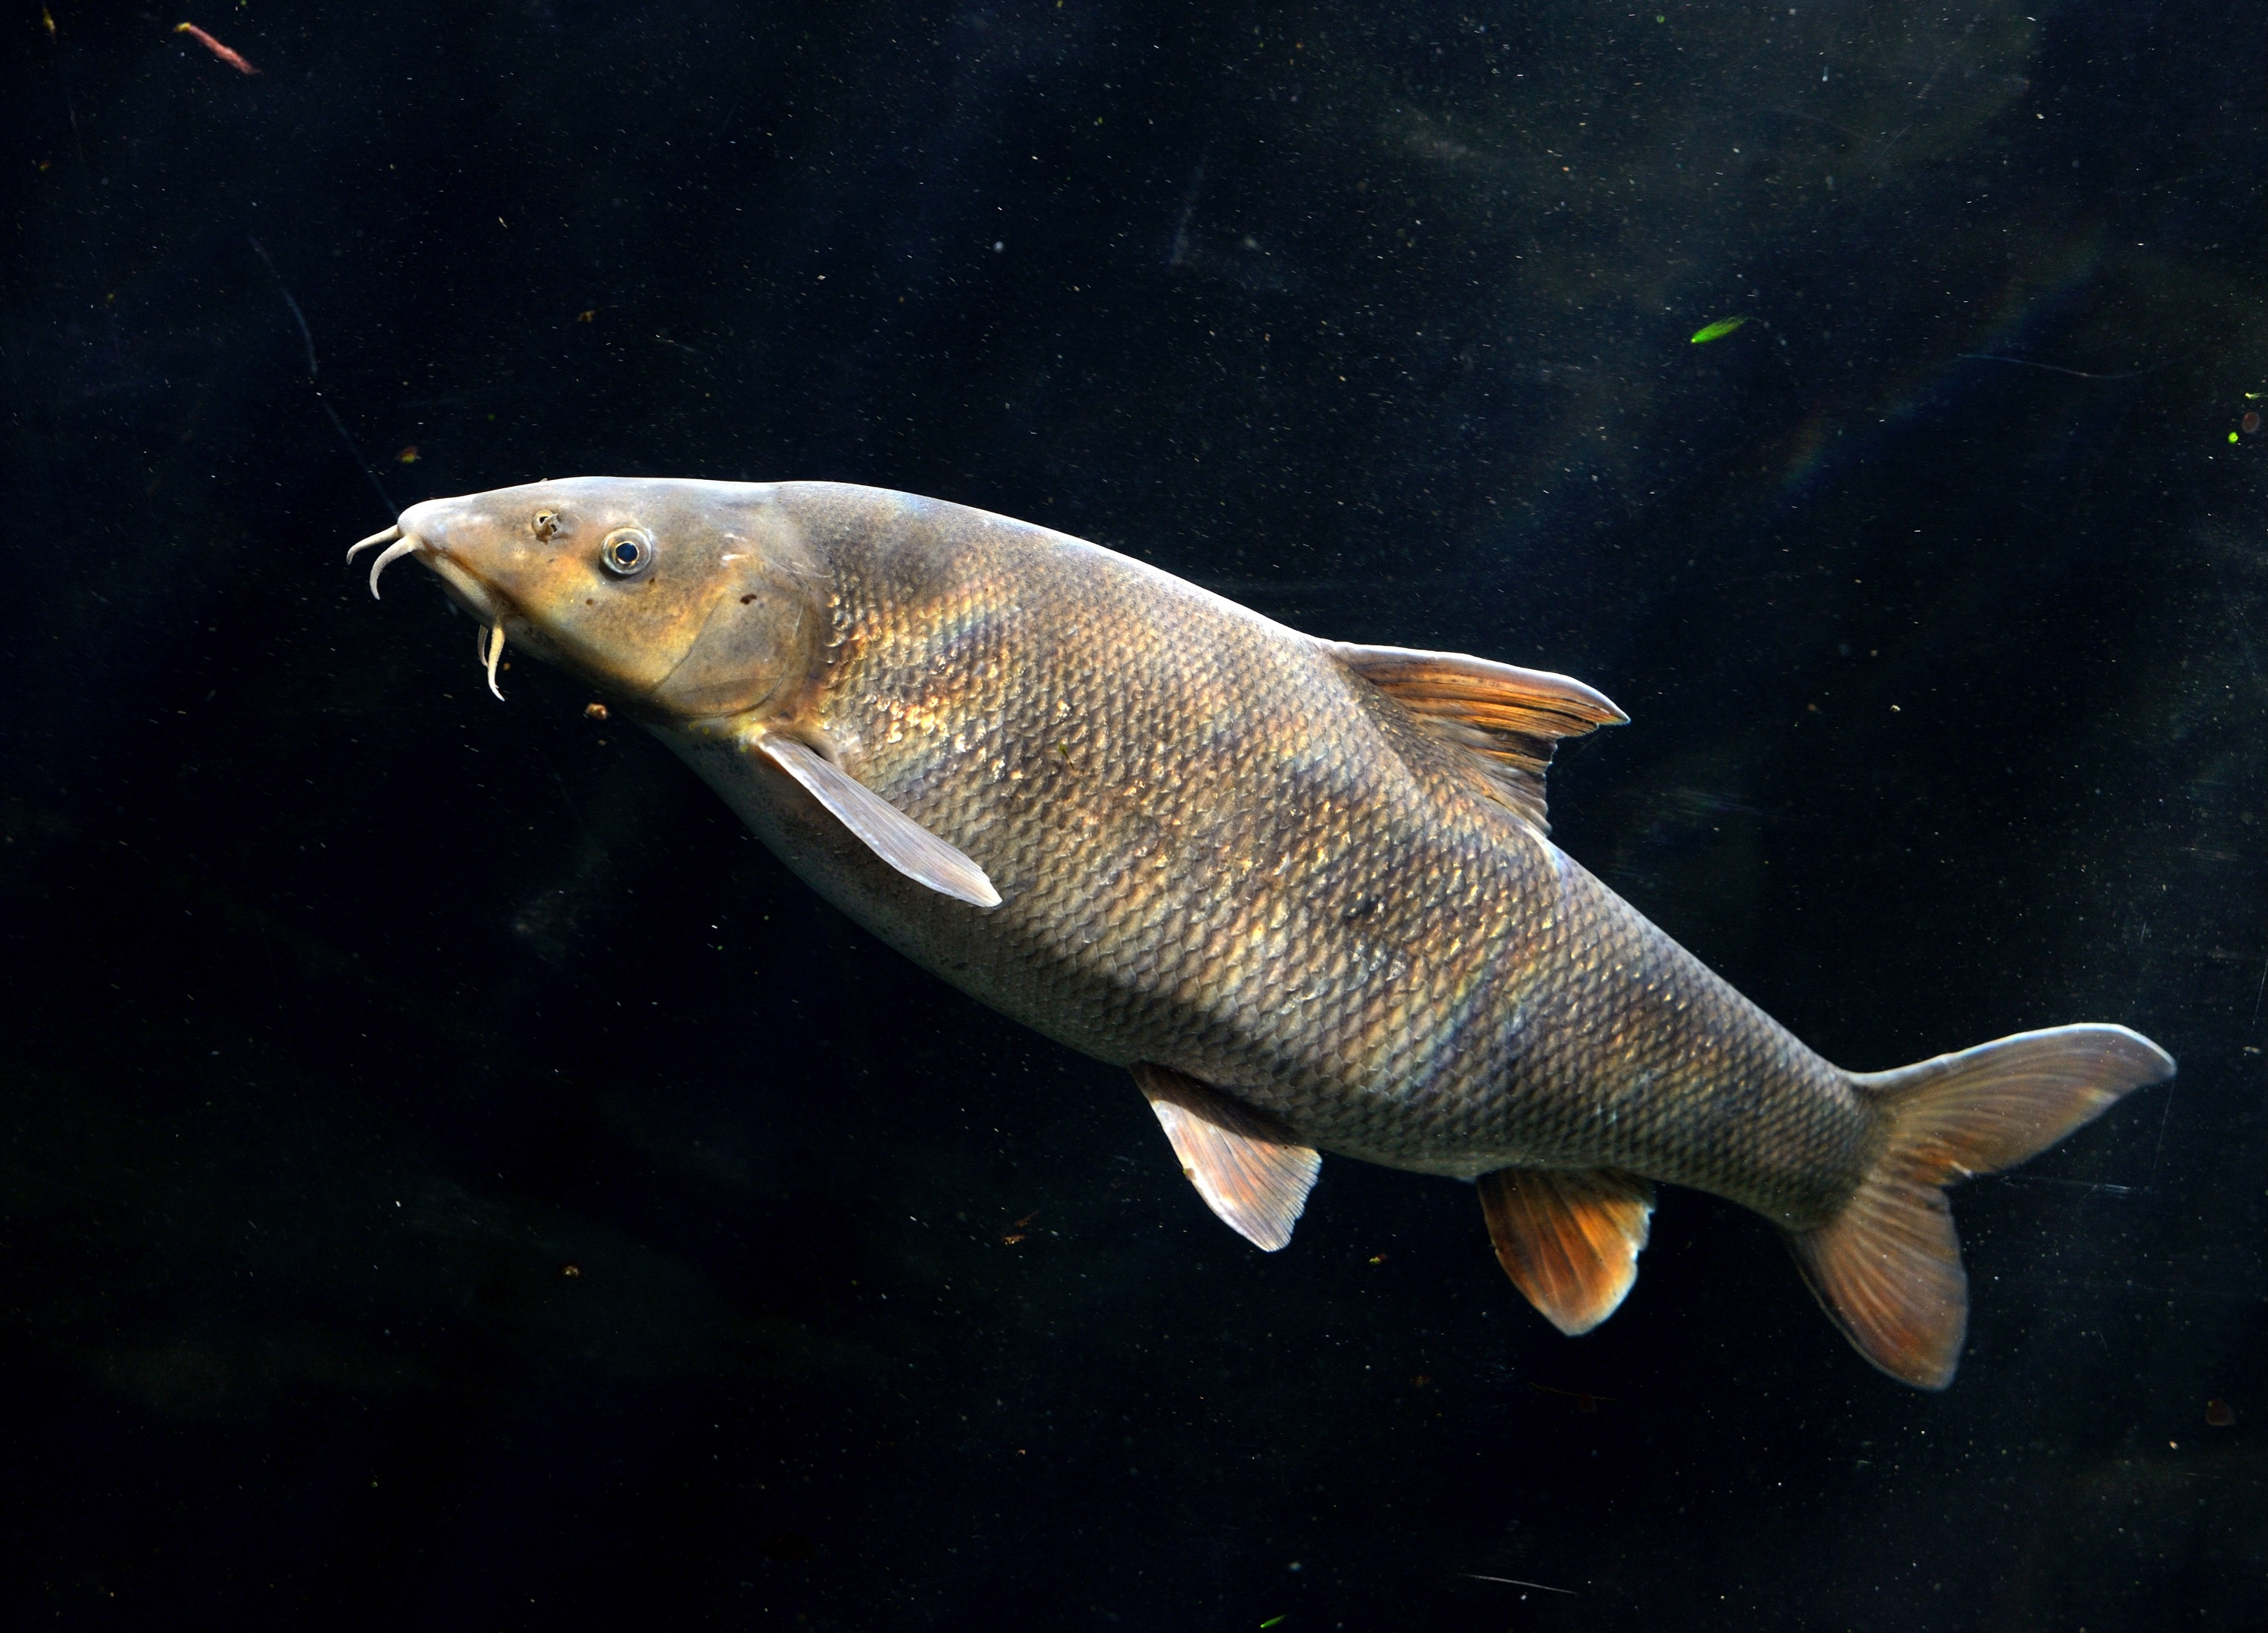
\includegraphics[height=4cm]{imagens/barbo.jpg}
        		\caption{\textit{Barbus barbus}}
       	 	\label{fig:barbo}
    		\end{subfigure}
    		
    		\caption{Familia Cyprinidae}
    		\label{fig:cypriniformes}
	\end{figure}

	\item \textbf{Ordem: Gadiformes}
	\begin{itemize}
		\item \textbf{Família: Gadidae}

A família Gadidae inclui peixes frequentemente encontrados em águas frias e profundas, como o Bacalhau-do-Atlântico (\textit{Gadus morhua}) (\ref{fig:bacalhau}) e o Elgefim (\textit{Melanogrammus aeglefinus}) (\ref{fig:elgefim}).
	\end{itemize}
	
	\begin{figure}[H]
	\center
    		\begin{subfigure}{.5\textwidth}
    		\center
        		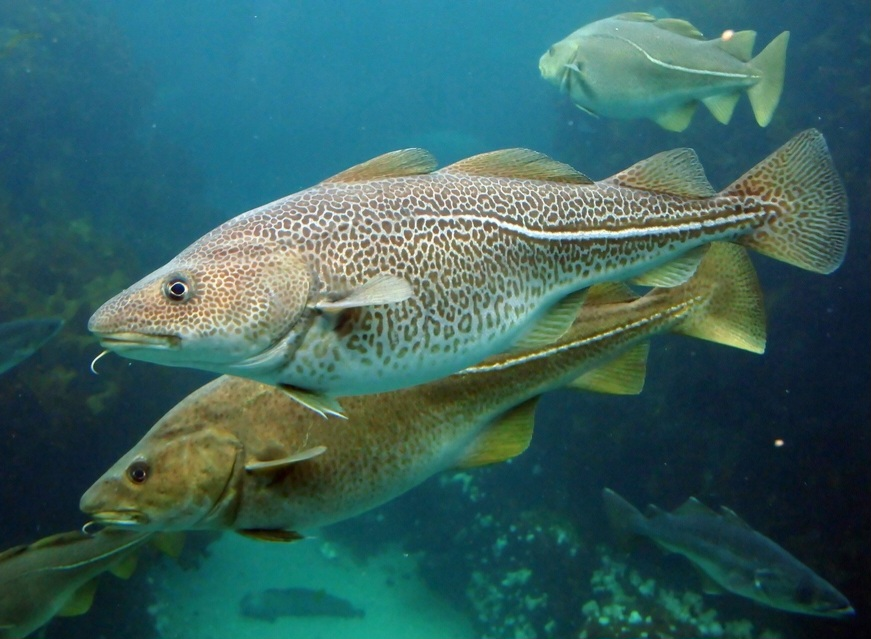
\includegraphics[height=4cm]{imagens/bacalhau.jpg}
        		\caption{\textit{Gadus morhua}}
        		\label{fig:bacalhau}
    		\end{subfigure}%
   		\begin{subfigure}{.5\textwidth}
    		\center
        		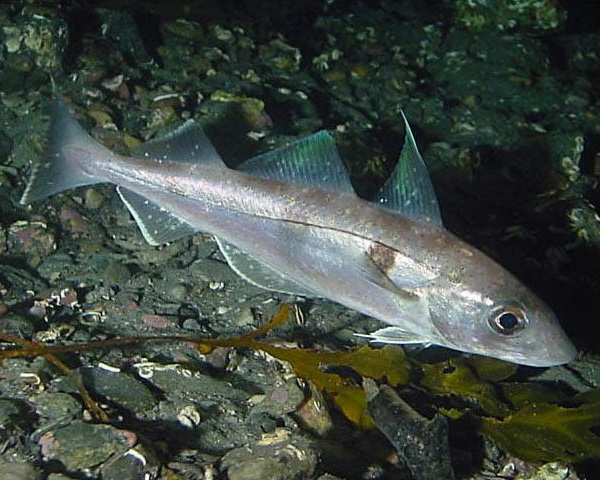
\includegraphics[height=4cm]{imagens/elgefim.jpg}
        		\caption{\textit{Melanogrammus aeglefinus}}
       	 	\label{fig:elgefim}
    		\end{subfigure}
    		
    		\caption{Familia Gadidae}
    		\label{fig:gadiformes}
	\end{figure}
	
	
	
	\item \textbf{Ordem: Syngnathiformes}
	\begin{itemize}
		\item \textbf{Família: Syngnathidae}
		
A família Syngnathidae destaca-se pela sua singularidade no reino dos peixes, especialmente devido ao papel invertido na gestação, como é o caso do Cavalo-marinho-comum (\textit{Hippocampus kuda}) (\ref{fig:cavalomarinho}).
	\end{itemize}
	
	\begin{figure}[H]
	\center
        	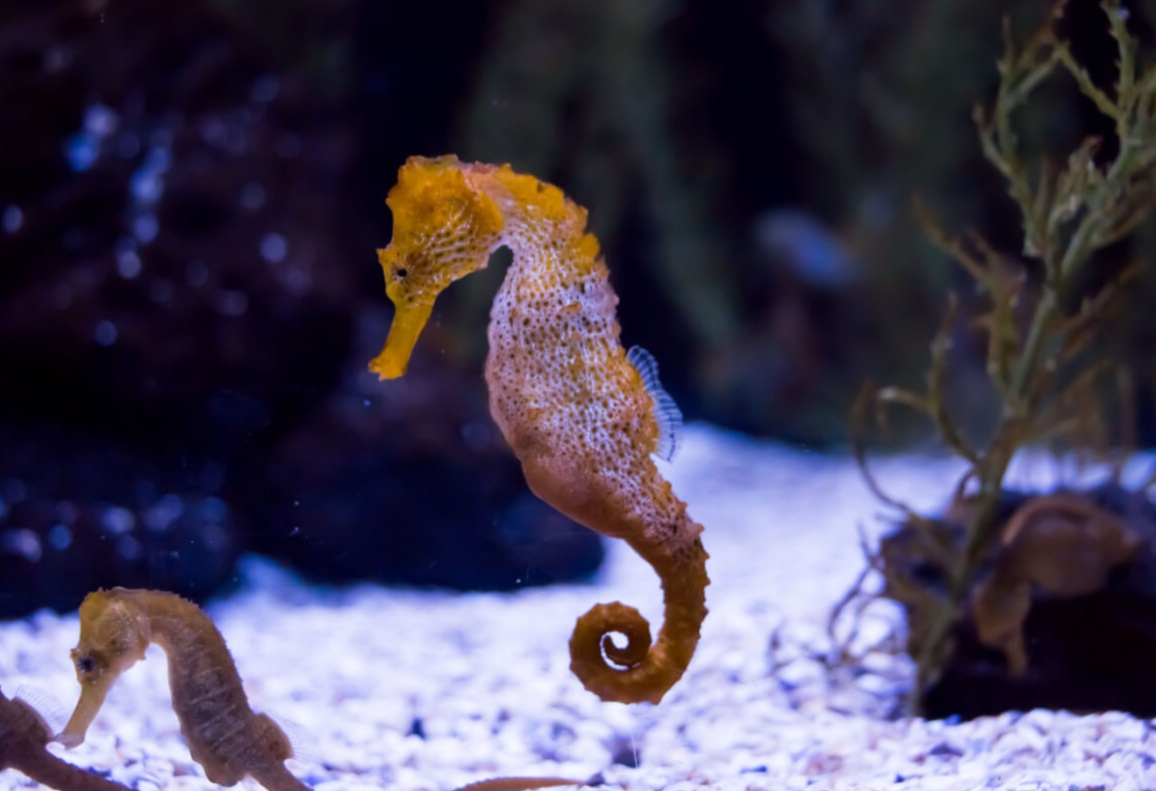
\includegraphics[height=4cm]{imagens/cavalomarinho.jpg}
        	\caption{\textit{Hippocampus kuda}}
        	\label{fig:cavalomarinho}
	\end{figure}	
\end{enumerate}

\subsection{Peixes Cartilaginosos (Chondrichthyes)}
\subsubsection{Anatomia e Morfologia}
Os peixes cartilaginosos, pertencentes à classe \textit{Chondrichthyes}, apresentam características anatómicas e morfológicas distintas que contribuem para a sua adaptação ao ambiente aquático. Essas características incluem:
\begin{itemize}
	\item \textbf{Esqueleto Cartilaginoso}: Ao contrário dos peixes ósseos, os peixes cartilaginosos possuem um esqueleto composto principalmente por cartilagem, tornando-os mais leves e ágeis na água. Isso também contribui para a sua flutuabilidade neutra, ou seja, os peixes cartilaginosos podem manter uma posição na coluna de água sem afundar ou flutuar involuntariamente.
	
	\item \textbf{Barbatanas especiais}: As barbatanas dos peixes cartilaginosos desempenham papéis específicos. A nadadeira dorsal é geralmente bem desenvolvida, que serve para estabilidade lateral. Algumas espécies, como os tubarões-martelo, possuem nadadeiras peitorais largas que facilitam manobras rápidas e precisas.
	
	\item \textbf{Pele sem Escamas}: Ao contrário dos peixes ósseos, os peixes cartilaginosos não possuem escamas. A pele é coberta por pequenas placas dérmicas chamadas dentículos dérmicos, que têm uma textura áspera, proporcionando resistência e eficiência hidrodinâmica.
	
	\item \textbf{Mandíbulas Poderosas e Dentes Substituíveis}: As mandíbulas dos peixes cartilaginosos são altamente móveis e dotadas de dentes afiados adaptadas para um estilo de vida de predador. Muitas espécies têm a capacidade de substituir rapidamente os dentes perdidos, garantindo uma funcionalidade contínua.
	
	\item \textbf{Fendas Braquiais Expostas}: Ao contrário dos peixes ósseos, cujas fendas braquiais são protegidas pelo óperculo, os peixes cartilaginosos apresentam fendas braquiais diretamente expostas ao meio ambiente aquático.
\end{itemize} 

\subsubsection{Classificação Taxonómica}
\begin{enumerate}
	\item \textbf{Ordem Torpediniformes}
	\begin{itemize}
		\item \textbf{Família: Torpedinidae}
		
Esta família é conhecida pela sua capacidade única de produzir descargas elétricas, como por exemplo a raia elétrica (\textit{Torpedo californica}) (\ref{fig:raiaeletrica}).
	\end{itemize}
	
	\begin{figure}[H]
	\center
        	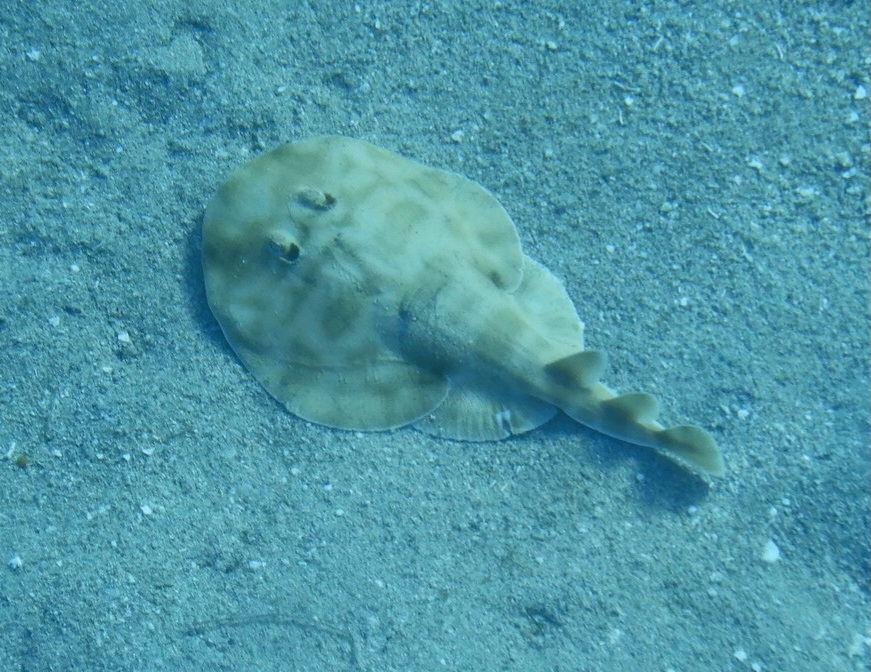
\includegraphics[height=4cm]{imagens/raiaeletrica.jpg}
        	\caption{\textit{Torpedo californica}}
        	\label{fig:raiaeletrica}
	\end{figure}	


	\item \textbf{Ordem: Myliobatiformes}
	\begin{itemize}
		\item \textbf{Família: Myliobatidae}
		
As mantas pertencem à família Myliobatidae (\textit{Mobula birostris}) (\ref{fig:manta}) e são conhecidas pelas suas barbatanas em forma de asa.
	\end{itemize}
	
	\begin{figure}[H]
	\center
        	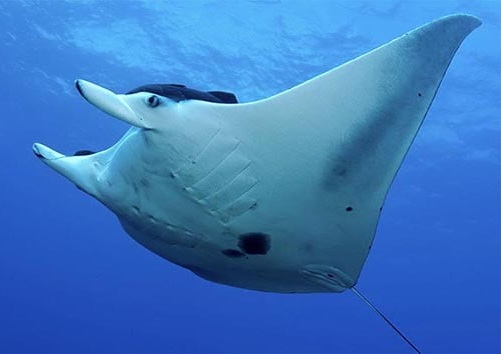
\includegraphics[height=4cm]{imagens/manta.jpg}
        	\caption{\textit{Mobula birostris}}
        	\label{fig:manta}
	\end{figure}
	
	\item \textbf{Ordem: Lamniformes}
	\begin{itemize}
		\item \textbf{Família: Lamnidae}
		
Os tubarões da família Lamnidae como o tubarão-branco (\textit{Carcharodon carcharias}) (\ref{fig:tubaraobranco}) e o tubarão-mako (\textit{Isurus oxyrinchus}) (\ref{fig:tubaraomako}) são conhecidos pelas suas incríveis capacidades de caça, são grandes predadores, adaptados para nadar rapidamente e capturar presas ágeis.
	\end{itemize}
	
	\begin{figure}[H]
	\center
    		\begin{subfigure}{.5\textwidth}
    		\center
        		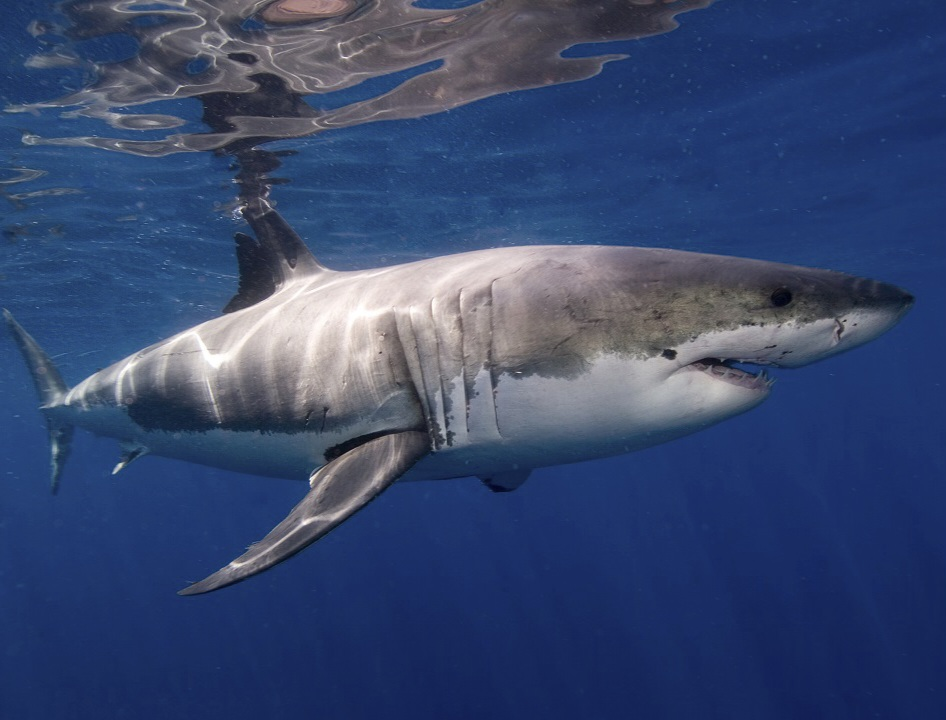
\includegraphics[height=4cm]{imagens/tubaraobranco.jpg}
        		\caption{\textit{Carcharodon carcharias}}
        		\label{fig:tubaraobranco}
    		\end{subfigure}%
   		\begin{subfigure}{.5\textwidth}
    		\center
        		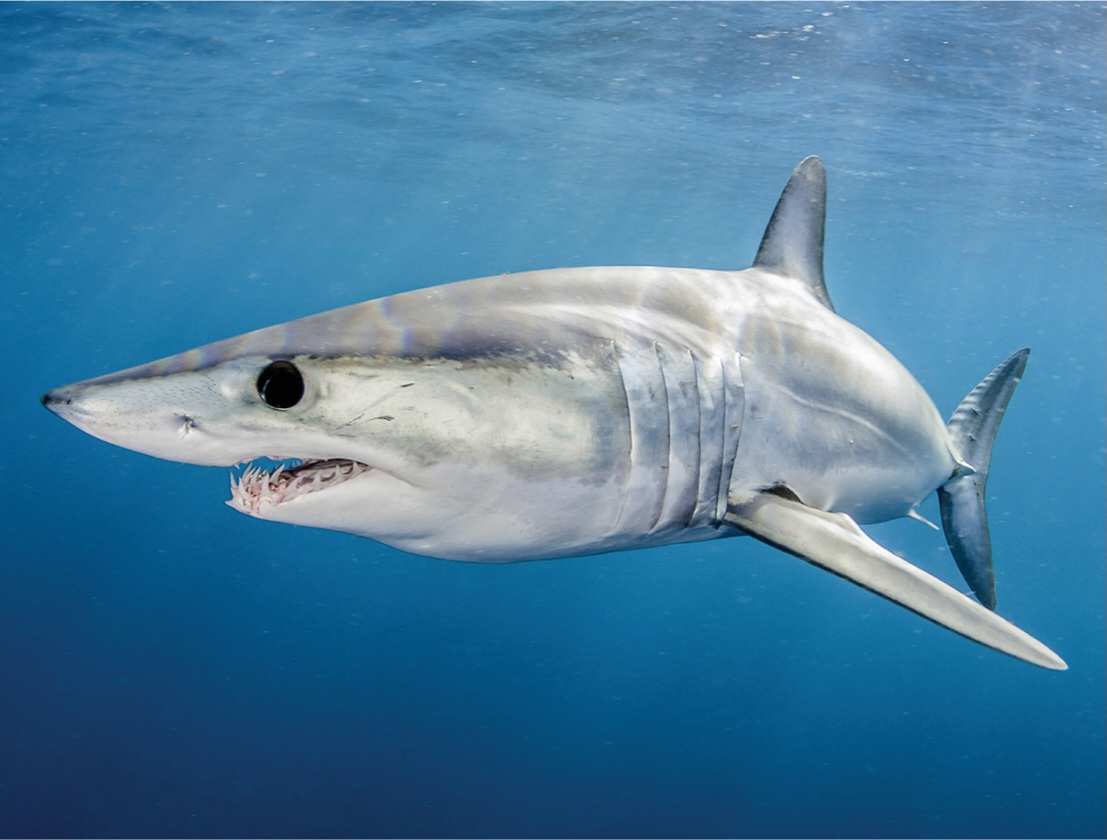
\includegraphics[height=4cm]{imagens/tubaraomako.jpg}
        		\caption{\textit{Isurus oxyrinchus}}
       	 	\label{fig:tubaraomako}
    		\end{subfigure}
    		\caption{Familia Lamnidae}
    		\label{fig:lamnidae}
	\end{figure}
	
	\item \textbf{Ordem: Orectolobiformes}
	\begin{itemize}
		\item \textbf{Família: Rhincodontidae}
		
Os tubarões baleia (\textit{Rhincodon typus}) (\ref{fig:tubaraobaleia}) da família  Rhincodontidae são os maiores tubarões do mundo, com cabeças largas e bocas enormes, alimentam-se principalmente de plâncton e pequenos peixes.
	\end{itemize}
	
	\begin{figure}[H]
	\center
        	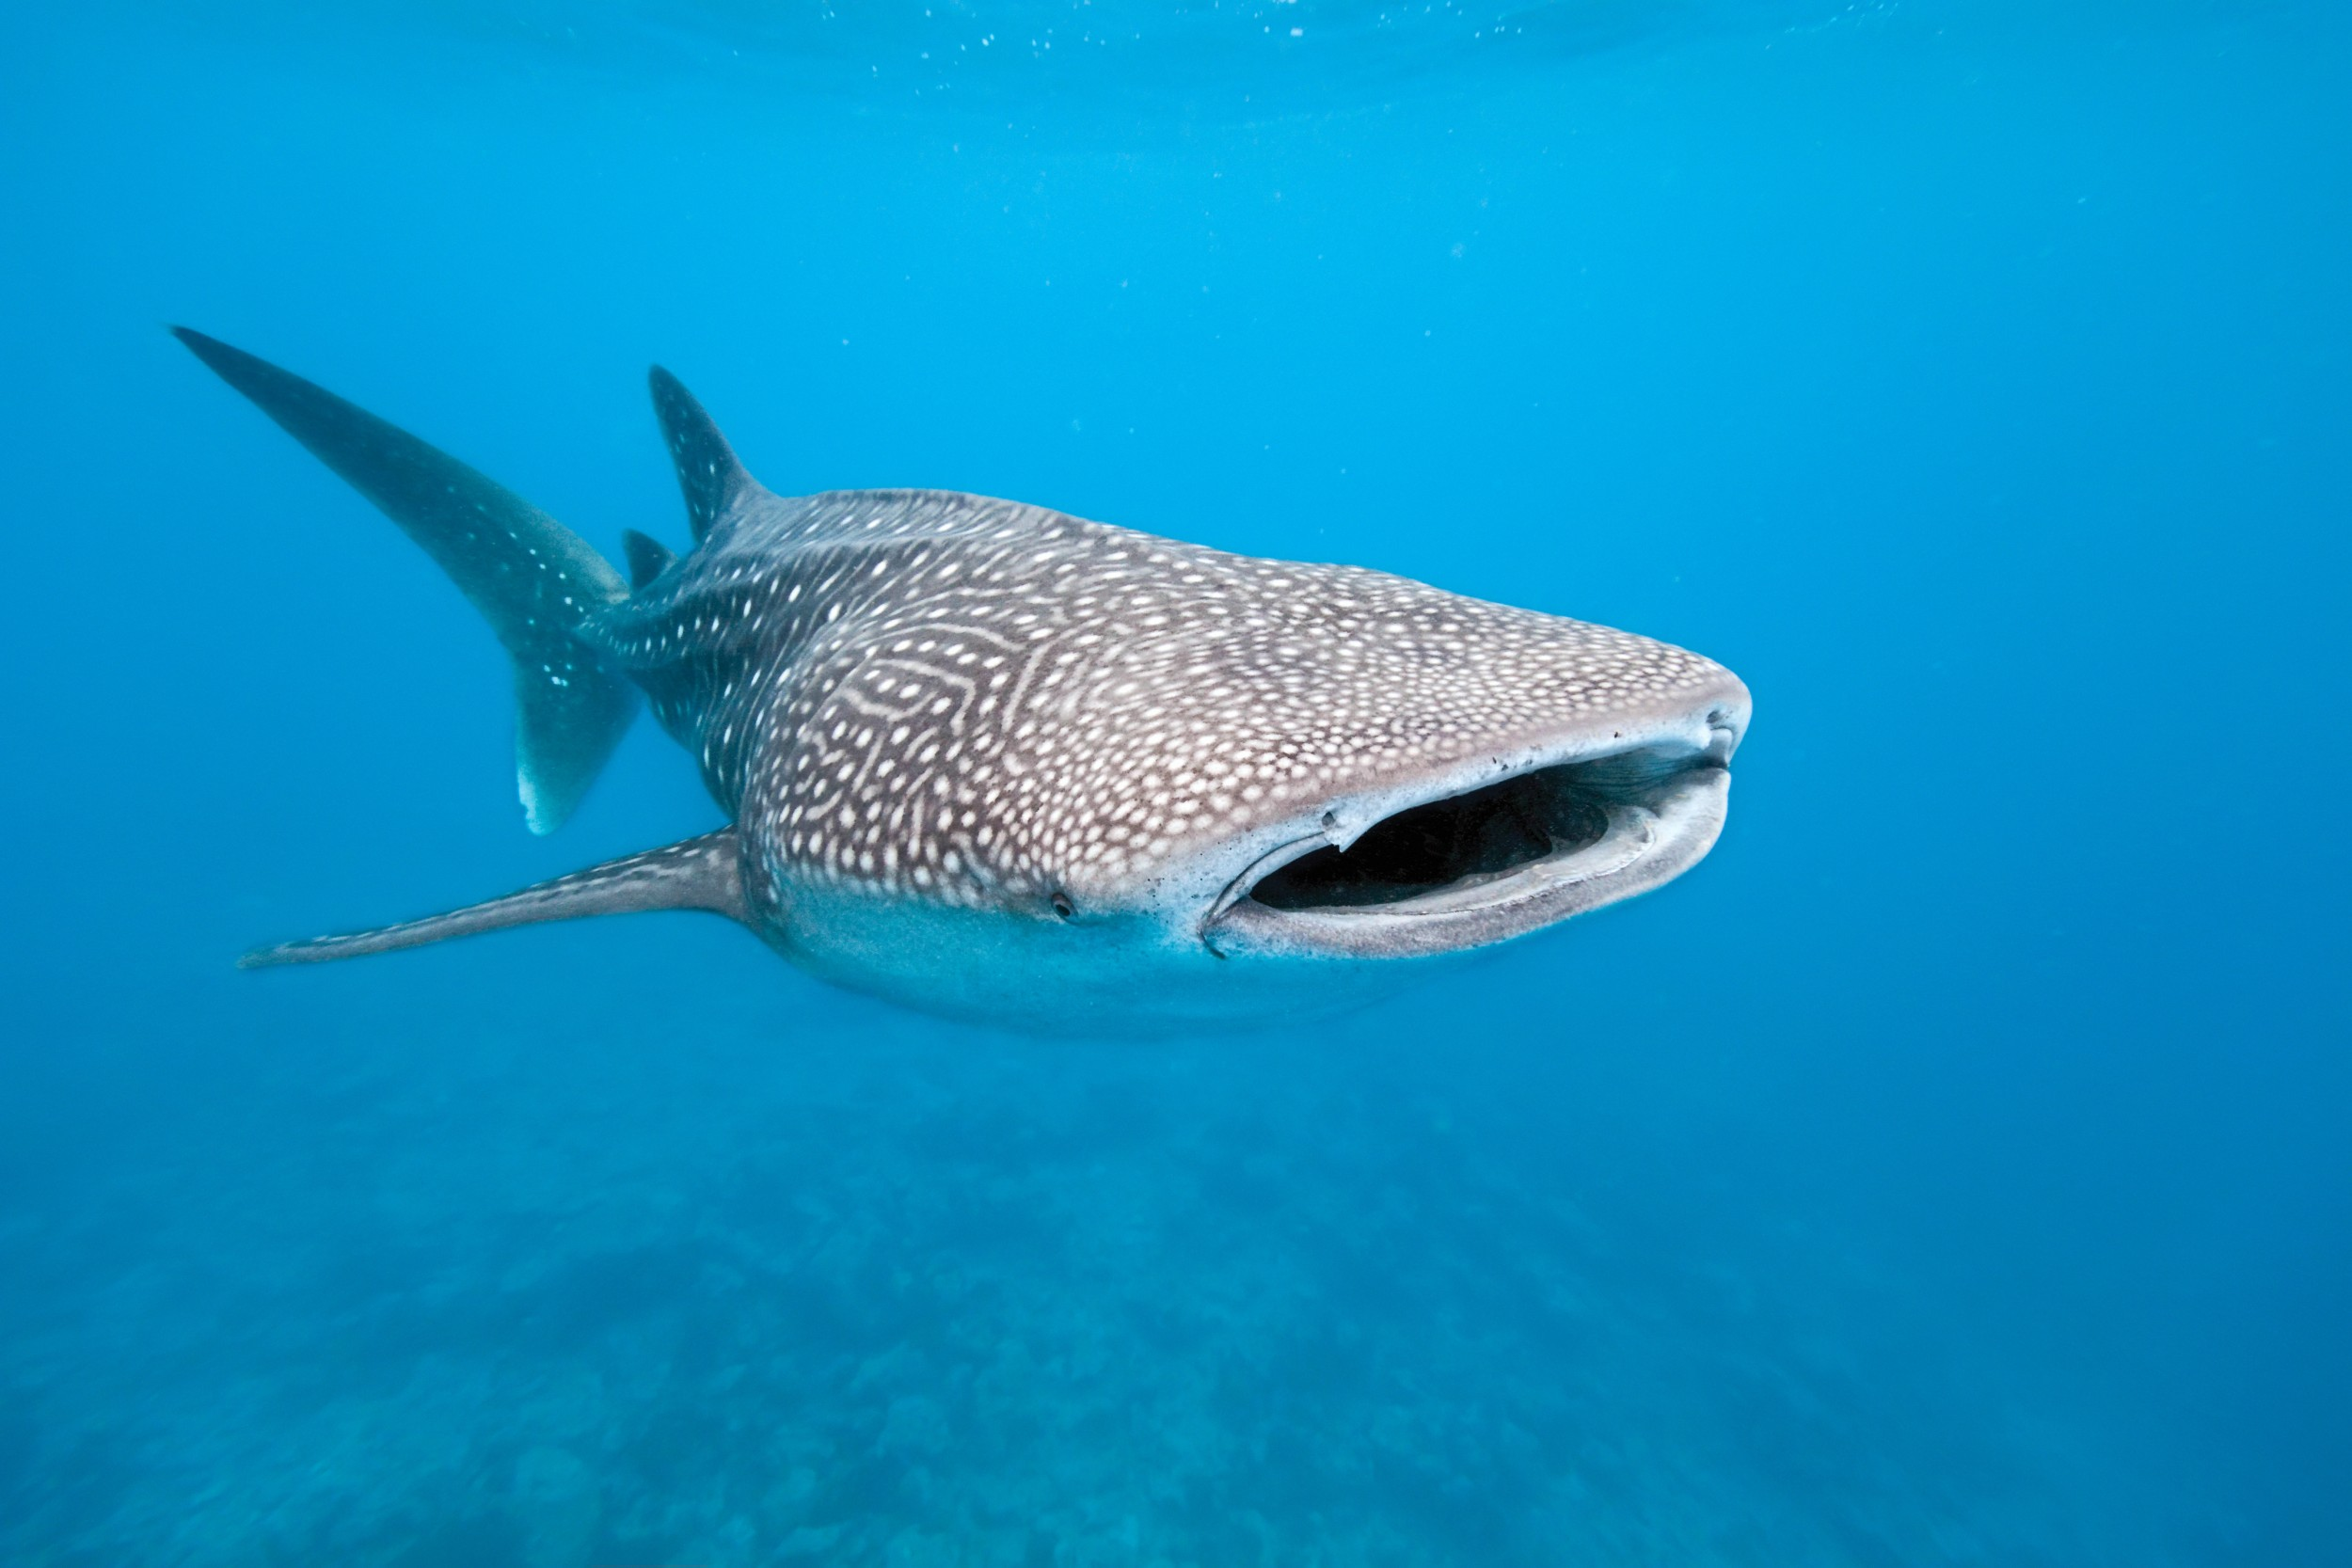
\includegraphics[height=4cm]{imagens/tubaraobaleia.jpg}
        	\caption{\textit{Rhincodon typus}}
        	\label{fig:tubaraobaleia}
	\end{figure}
	
\end{enumerate}

\section{Mamíferos}
\subsection{Cetáceos}
Os cetáceos constituem uma ordem de mamíferos marinhos caracterizado por corpos adaptados à vida aquática. Essa ordem é dividida em três principais grupos: baleias, golfinhos e botos


\subsubsection{Baleias}
As baleias apresentam tamanhos variados, desde da baleia-azul (\ref{fig:baleiaazul}), que é considerada o maior animal do planeta, até a algumas mais pequenas como a baleia-cinzenta (\ref{fig:baleiacinzenta}). Algumas como a baleia-jubarte (\ref{fig:baleiajubarte}) são conhecidas pelos seus saltos espetaculares.

\begin{figure}[H]
\center
    \begin{subfigure}{.5\textwidth}
    \center
        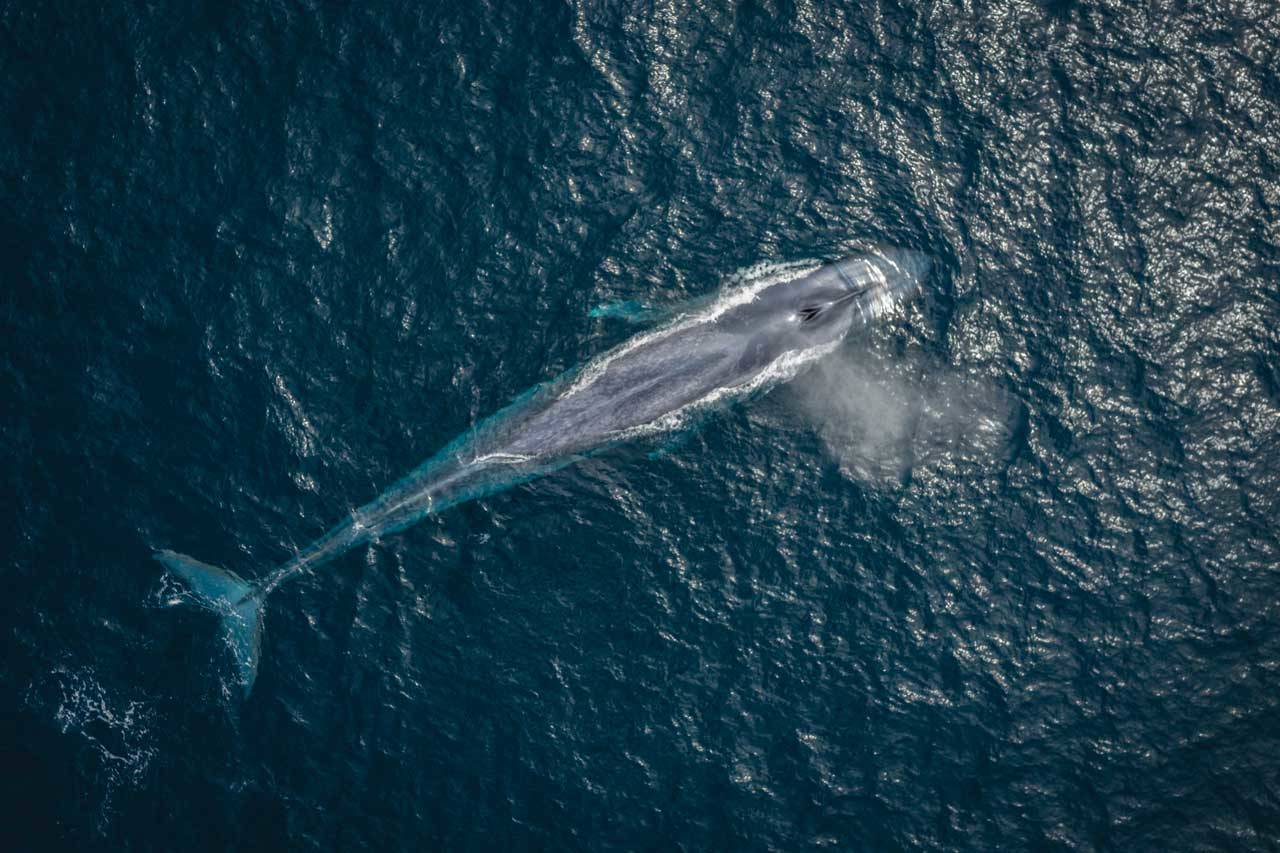
\includegraphics[height=4cm]{imagens/baleiaazul.jpg}
        \caption{Baleia azul}
        \label{fig:baleiaazul}
    \end{subfigure}%
    \hfill
    \begin{subfigure}{.5\textwidth}
    \center
        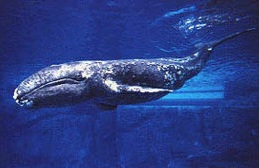
\includegraphics[height=4cm]{imagens/baleiacinzenta.jpg}
        \caption{baleia cinzenta}
        \label{fig:baleiacinzenta}
    \end{subfigure}%
    \hfill
    \begin{subfigure}{.5\textwidth}
    \center    
        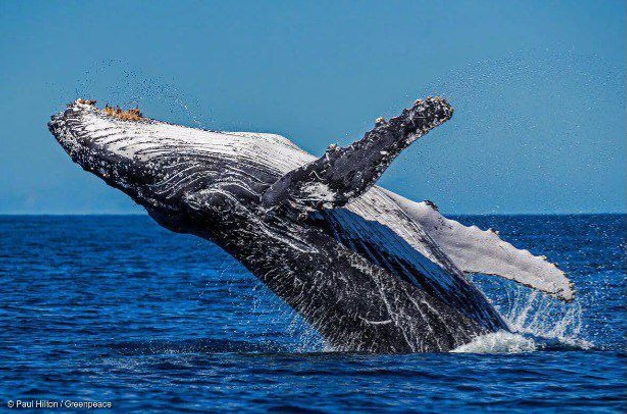
\includegraphics[height=4cm]{imagens/jubarte.jpg}
        \caption{baleia jubarte}
        \label{fig:baleiajubarte}
    \end{subfigure}
    \caption{Baleias}
    \label{fig:baleias}
\end{figure}

\subsubsection{Golfinhos e Botos}
Os golfinhos (\ref{fig:golfinho}) e botos (\ref{fig:boto}) são cetáceos menores que as baleias, conhecidos pela sua inteligência e comportamento complexo. São ágeis nadadores e exibem frequentemente acrobacias na água.

\begin{figure}[H]
\center
    	\begin{subfigure}{.5\textwidth}
    	\center
        	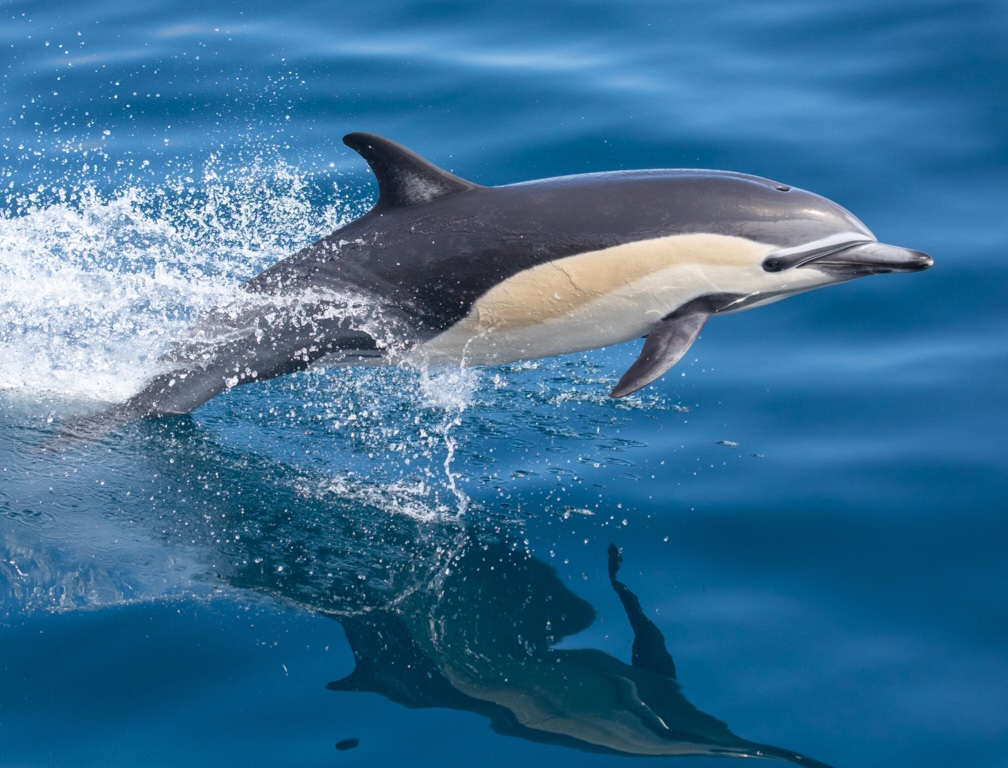
\includegraphics[height=4cm]{imagens/golfinhocomum.jpg}
        	\caption{Golfinho}
        	\label{fig:golfinho}
    	\end{subfigure}%
   	\begin{subfigure}{.5\textwidth}
    	\center
        	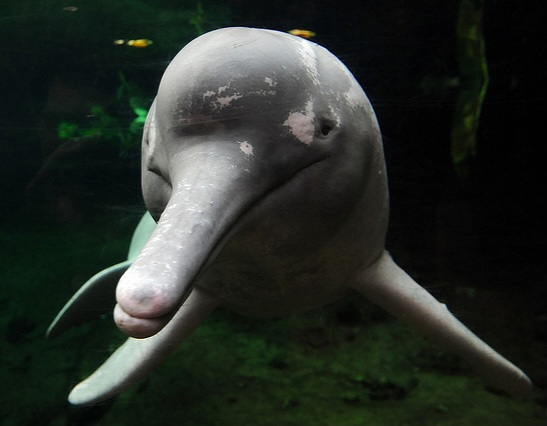
\includegraphics[height=4cm]{imagens/boto.jpg}
        	\caption{Boto}
       	\label{fig:boto}
    	\end{subfigure}
    \caption{Golfinhos e Botos}
    	\label{fig:golfinhosbotos}
\end{figure}
	

\subsection{Penípedes}
Os penípedes são mamíferos marinhos, que inclui focas, leões-marinhos e morsas. Eles apresentam adaptações físicas tanto para a vida em terra como no mar.

As focas (\ref{fig:foca}) distinguem-se pelos seus corpos alongados e focinhos curtos, nadam usando as barbatanas traseiras enquanto em terra movimentam-se com as barbatanas dianteiras.

Os leões-marinhos (\ref{fig:leaomarinho}) compartilham características com as focas, mas destacam-se pelos seus corpos robustos e orelhas externas.
	
As morsas (\ref{fig:morsa}) são conhecidas pelas suas longas e curvas presas, utilizadas para cavar no leito do mar em busca de alimento.


\begin{figure}[H]
\center
    \begin{subfigure}{.5\textwidth}
    \center
        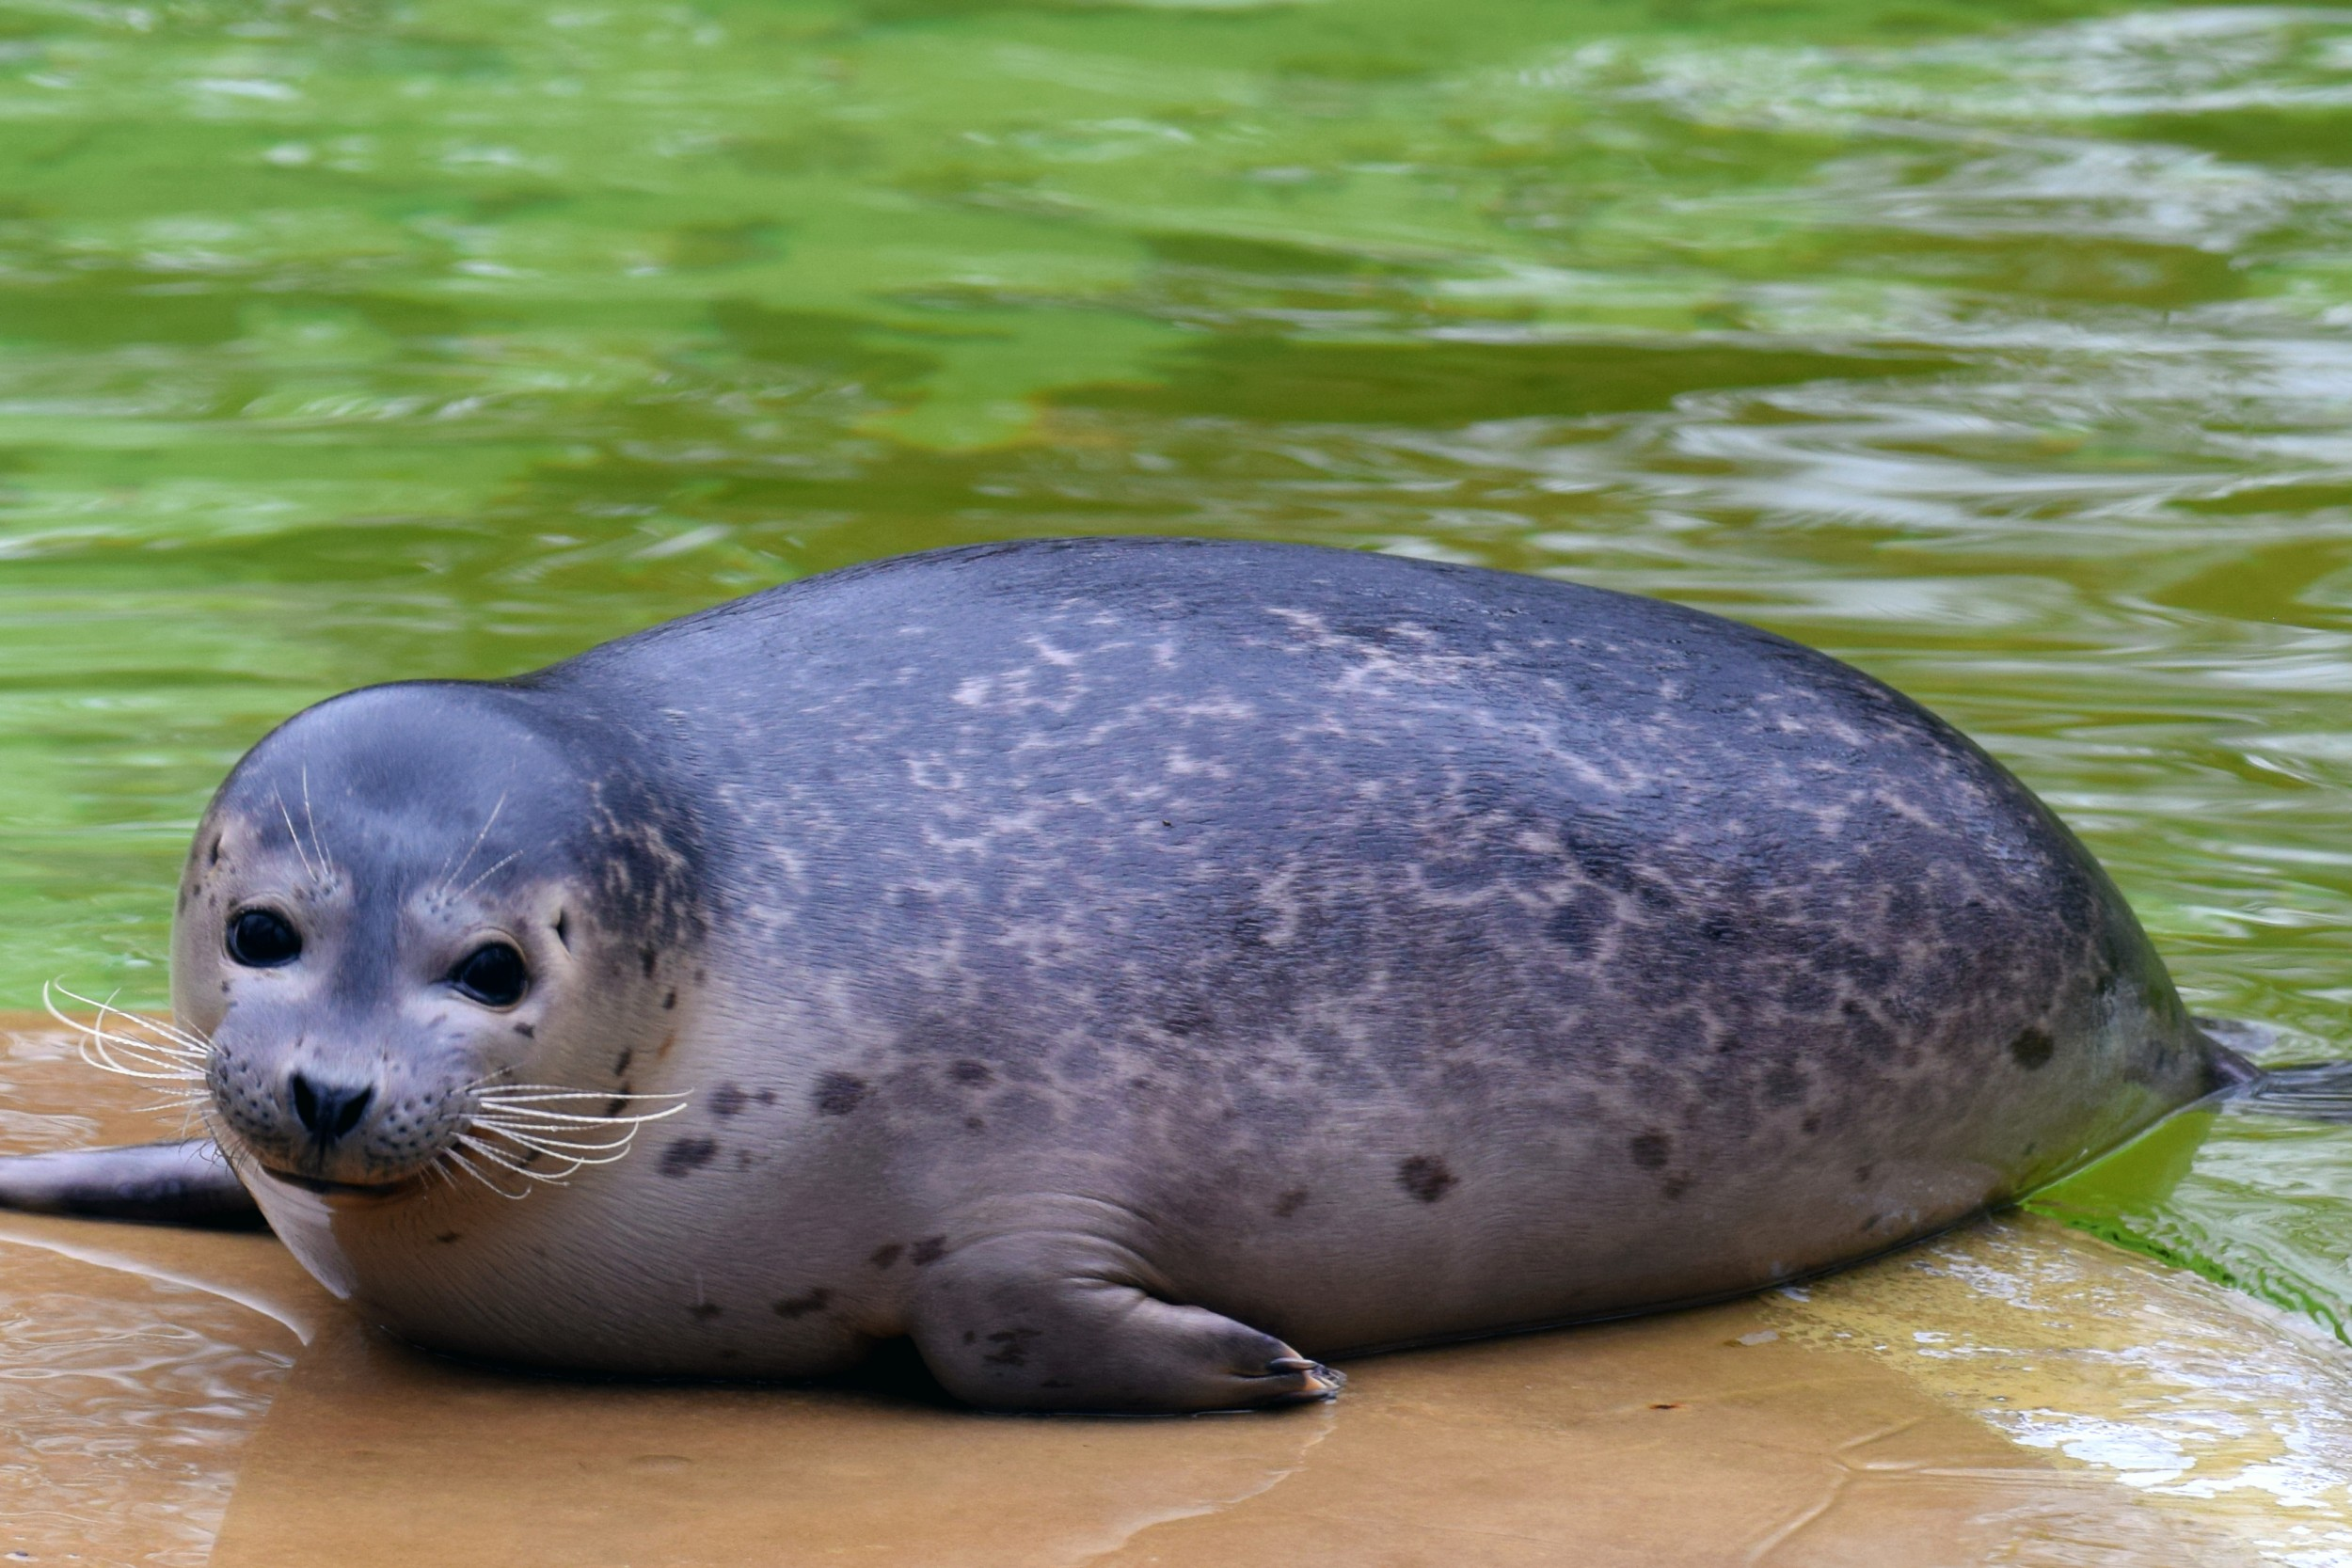
\includegraphics[height=4cm]{imagens/foca.jpg}
        \caption{Foca}
        \label{fig:foca}
    \end{subfigure}%
    \hfill
    \begin{subfigure}{.5\textwidth}
    \center
        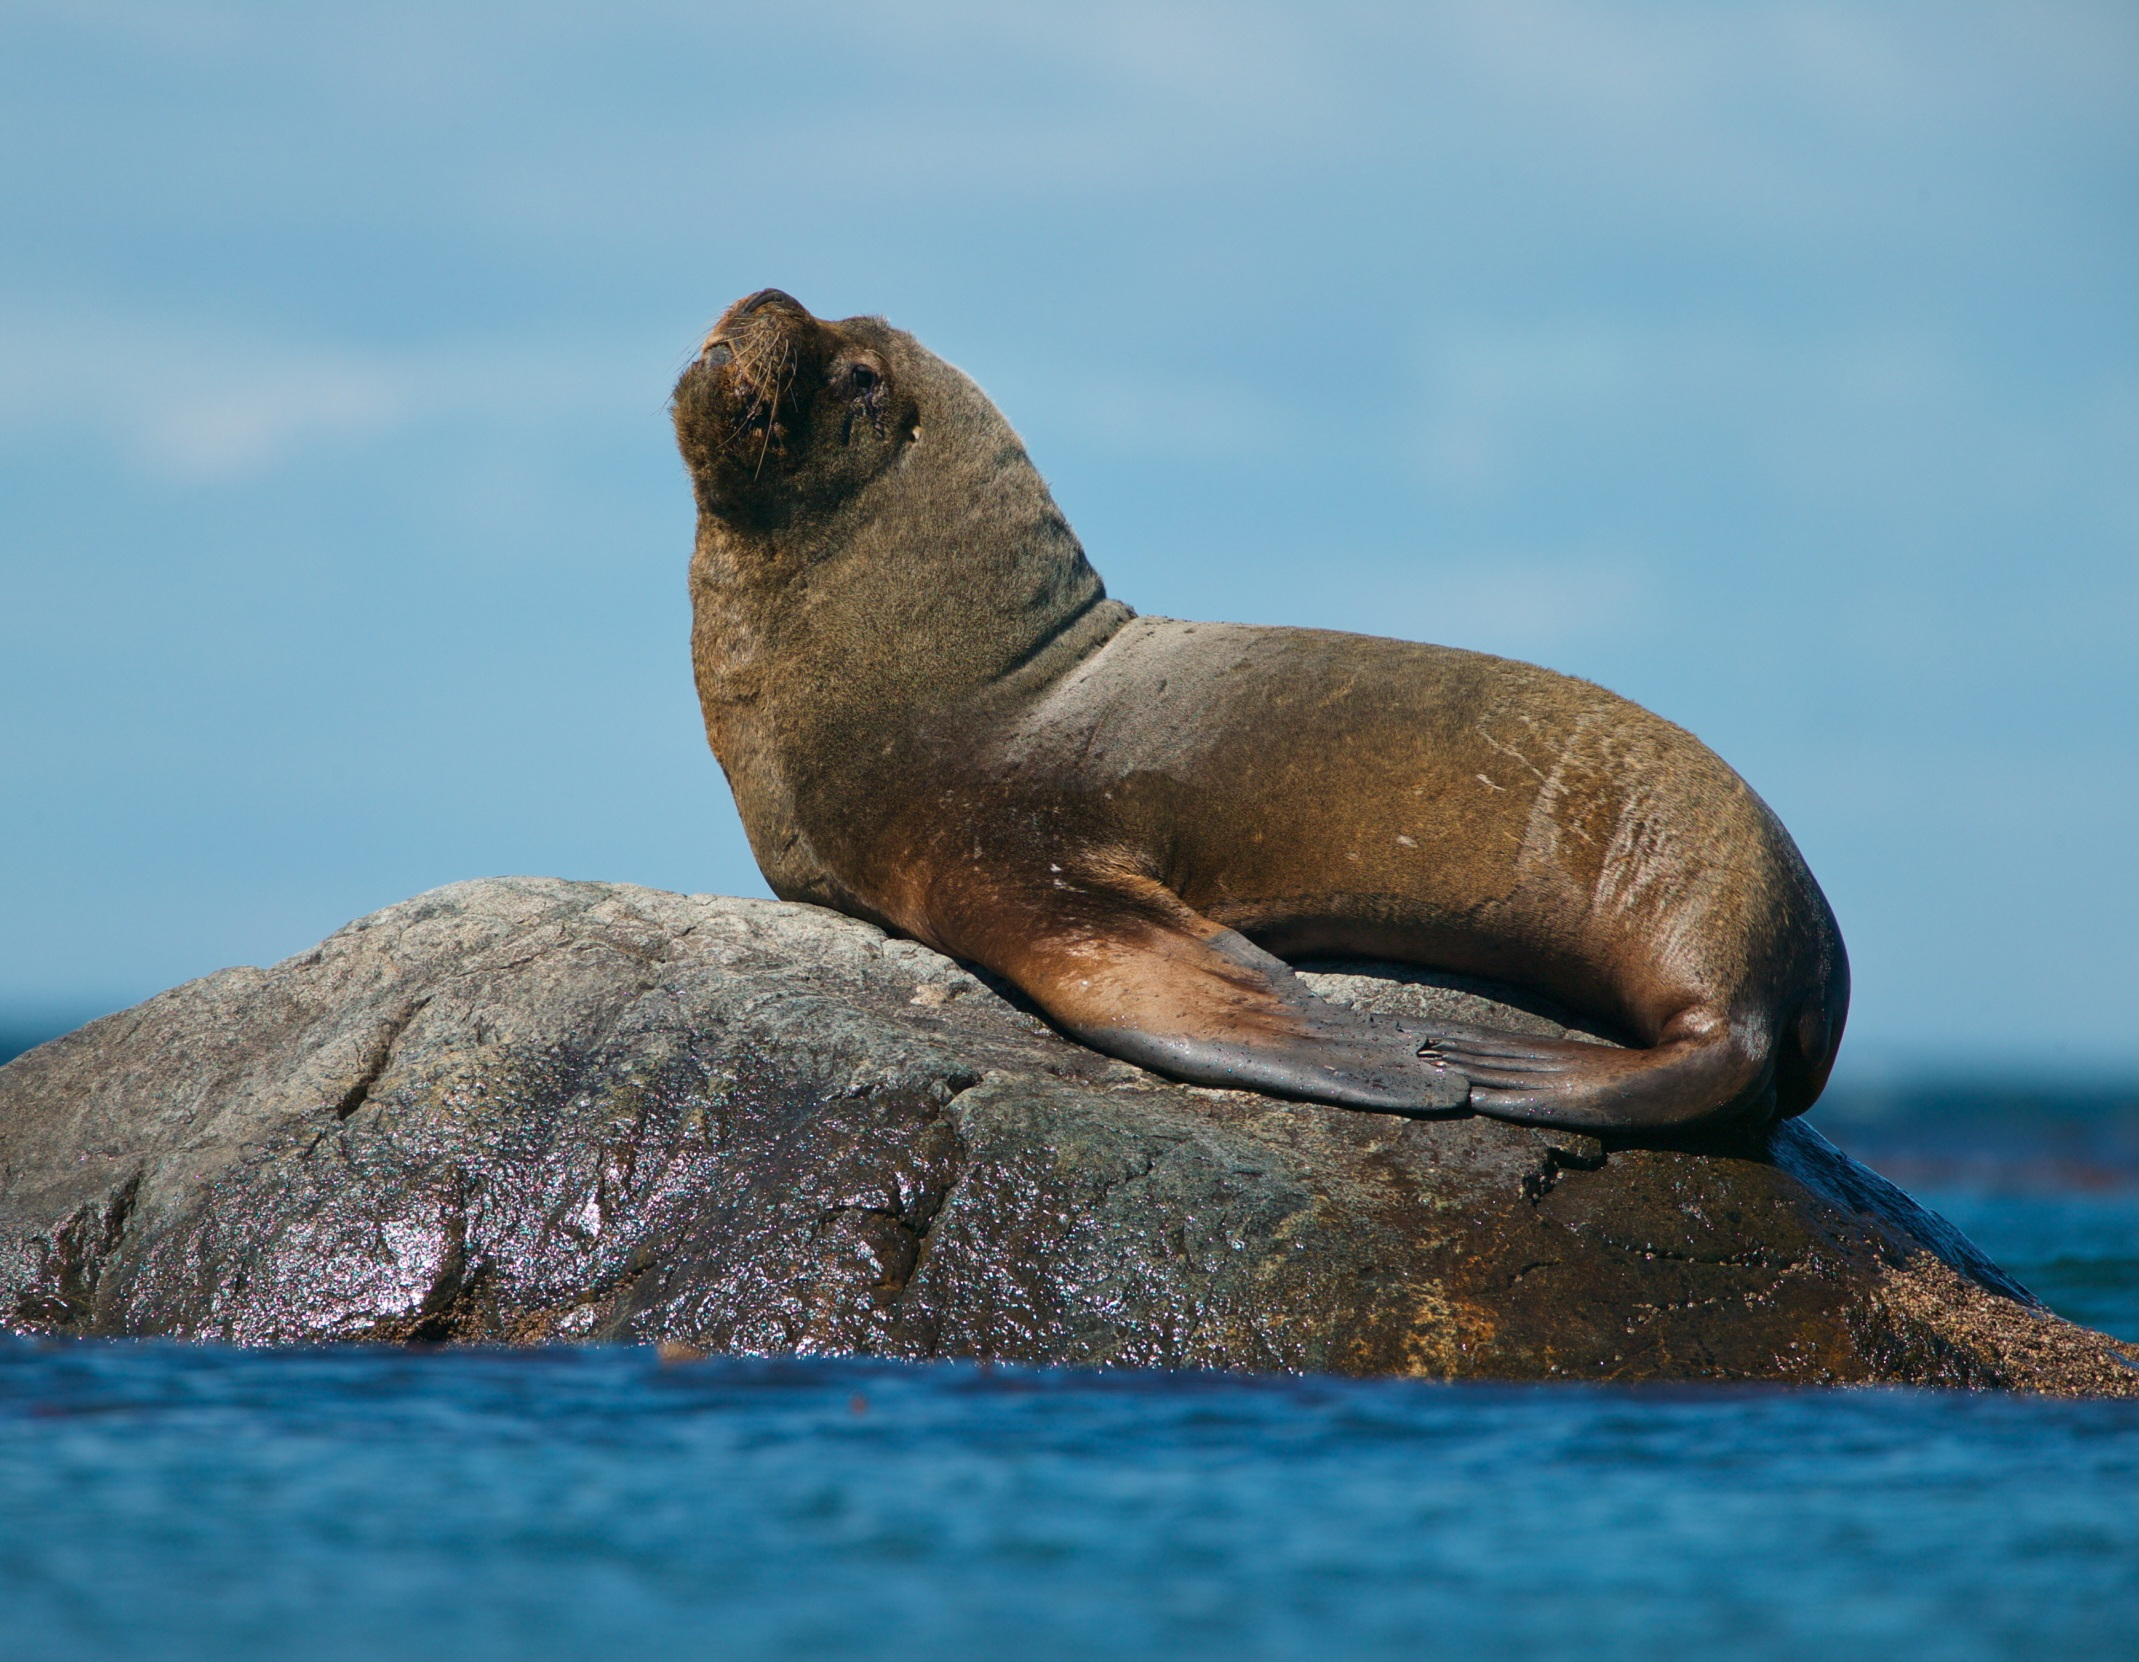
\includegraphics[height=4cm]{imagens/leaomarinho.jpg}
        \caption{Leão-marinho}
        \label{fig:leaomarinho}
    \end{subfigure}%
    \hfill
    \begin{subfigure}{.5\textwidth}
    \center    
        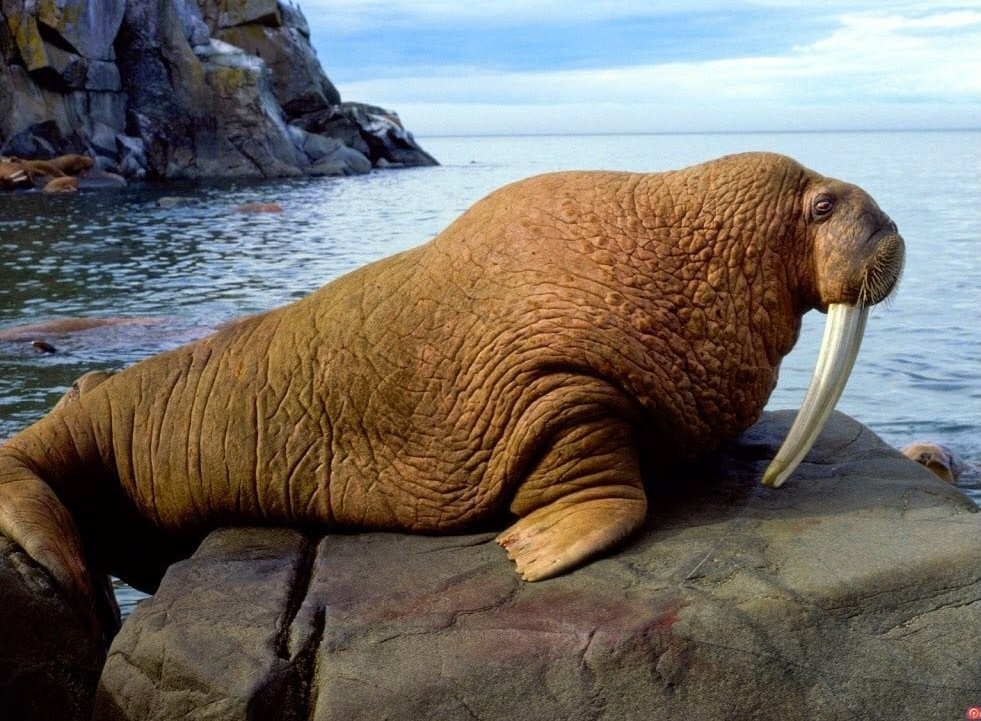
\includegraphics[height=4cm]{imagens/morsa.jpg}
        \caption{Morsa}
        \label{fig:morsa}
    \end{subfigure}
    \caption{Penípedes}
    \label{fig:penipedes}
\end{figure}

\section{Invertebrados}
\subsection{Moluscos}
\subsubsection{Cefalópodes}
Esta classe de moluscos inclui polvos (\ref{fig:polvo}), lulas (\ref{fig:lula}) e chocos (\ref{fig:choco}). Eles são conhecidos pelas suas habilidades de camuflagem e por serem predadores ágeis. Muitas espécies possuem uma inteligência surpreendente, especialmente os polvos.

\begin{figure}[H]
\center
    \begin{subfigure}{.5\textwidth}
    \center
        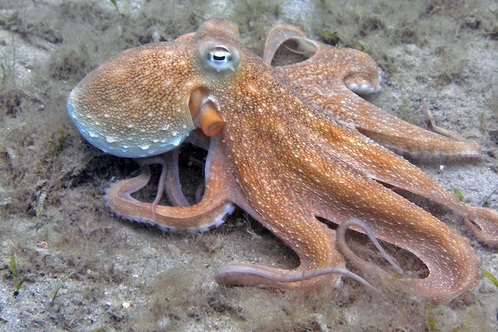
\includegraphics[height=4cm]{imagens/polvo.jpg}
        \caption{Polvo}
        \label{fig:polvo}
    \end{subfigure}%
    \hfill
    \begin{subfigure}{.5\textwidth}
    \center
        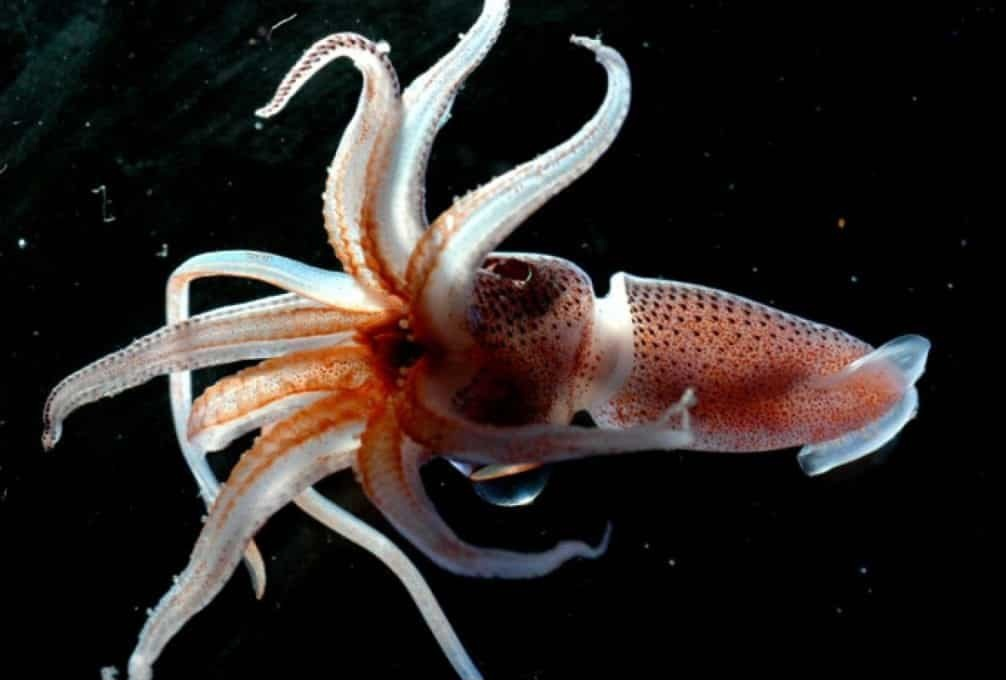
\includegraphics[height=4cm]{imagens/lula.jpg}
        \caption{Lula}
        \label{fig:lula}
    \end{subfigure}%
    \hfill
    \begin{subfigure}{.5\textwidth}
    \center    
        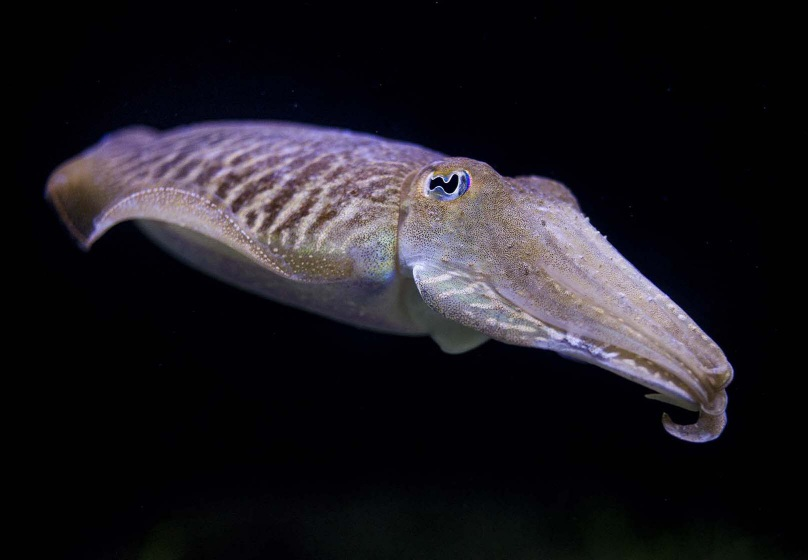
\includegraphics[height=4cm]{imagens/choco.jpg}
        \caption{Choco}
        \label{fig:choco}
    \end{subfigure}
    \caption{Cefalópodes}
    \label{fig:cefalopodes}
\end{figure}


\subsubsection{Bivalves}
Mexilhões (\ref{fig:mexilhao}), ostras (\ref{fig:ostra}) e vieiras são caracterizados por terem conchas formadas por duas partes, que se abrem e fecham, servindo igualmente de proteção para o corpo do molusco. Esta espécie filtra partículas da água para se alimentar.

\begin{figure}[H]
\center
    	\begin{subfigure}{.5\textwidth}
    	\center
        	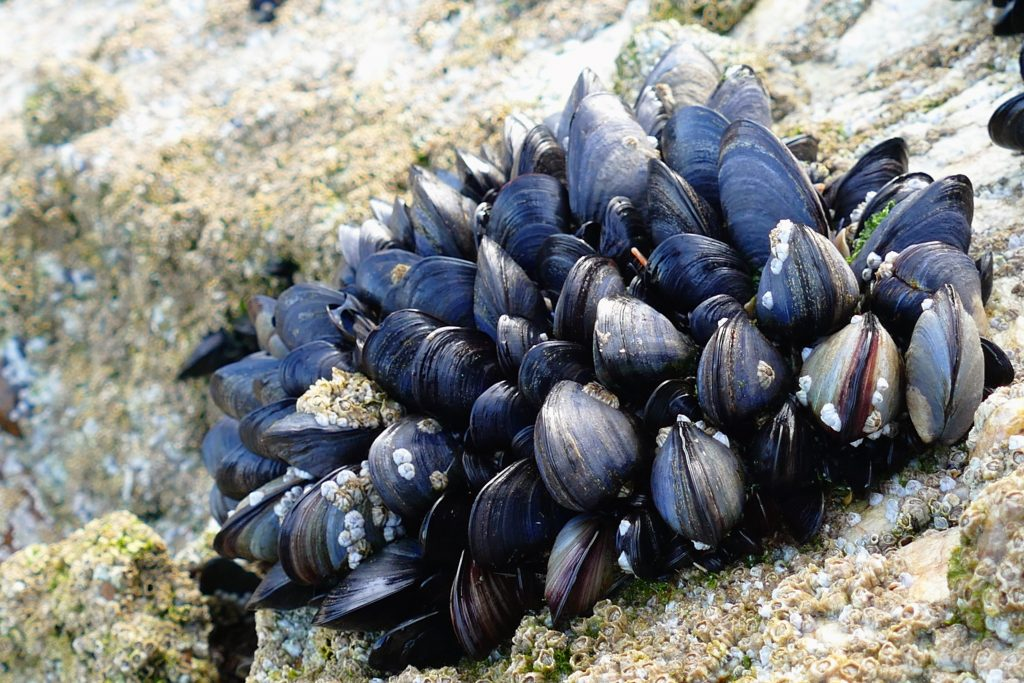
\includegraphics[height=4cm]{imagens/mexilhao.jpg}
        	\caption{Mexilhões}
        	\label{fig:mexilhao}
    	\end{subfigure}%
   	\begin{subfigure}{.5\textwidth}
    	\center
        	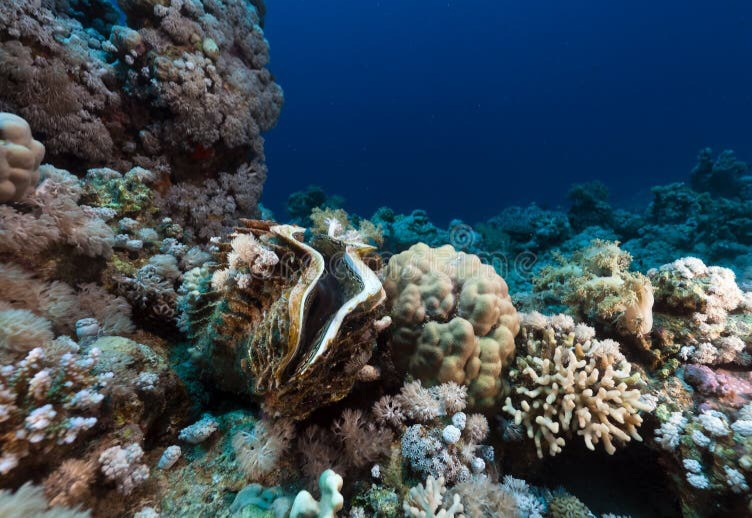
\includegraphics[height=4cm]{imagens/ostra.jpg}
        	\caption{Ostra}
       	\label{fig:ostra}
    	\end{subfigure}
    \caption{Bivalves}
    	\label{fig:bivalves}
\end{figure}

\subsubsection{Gastrópodes}
Estão incluídos nesta classe os caracóis marinhos, os búzios, as lapas (\ref{fig:lapas}) e as lesmas do mar (\ref{fig:lesma}). Muitas das conchas destes univalves, apresentam uma forma espiral e são encontrados em vários habitats marinhos, desde recifes de coral até praias arenosas e até mesmos nas rochas da orla marítima.

\begin{figure}[H]
\center
    	\begin{subfigure}{.5\textwidth}
    	\center
        	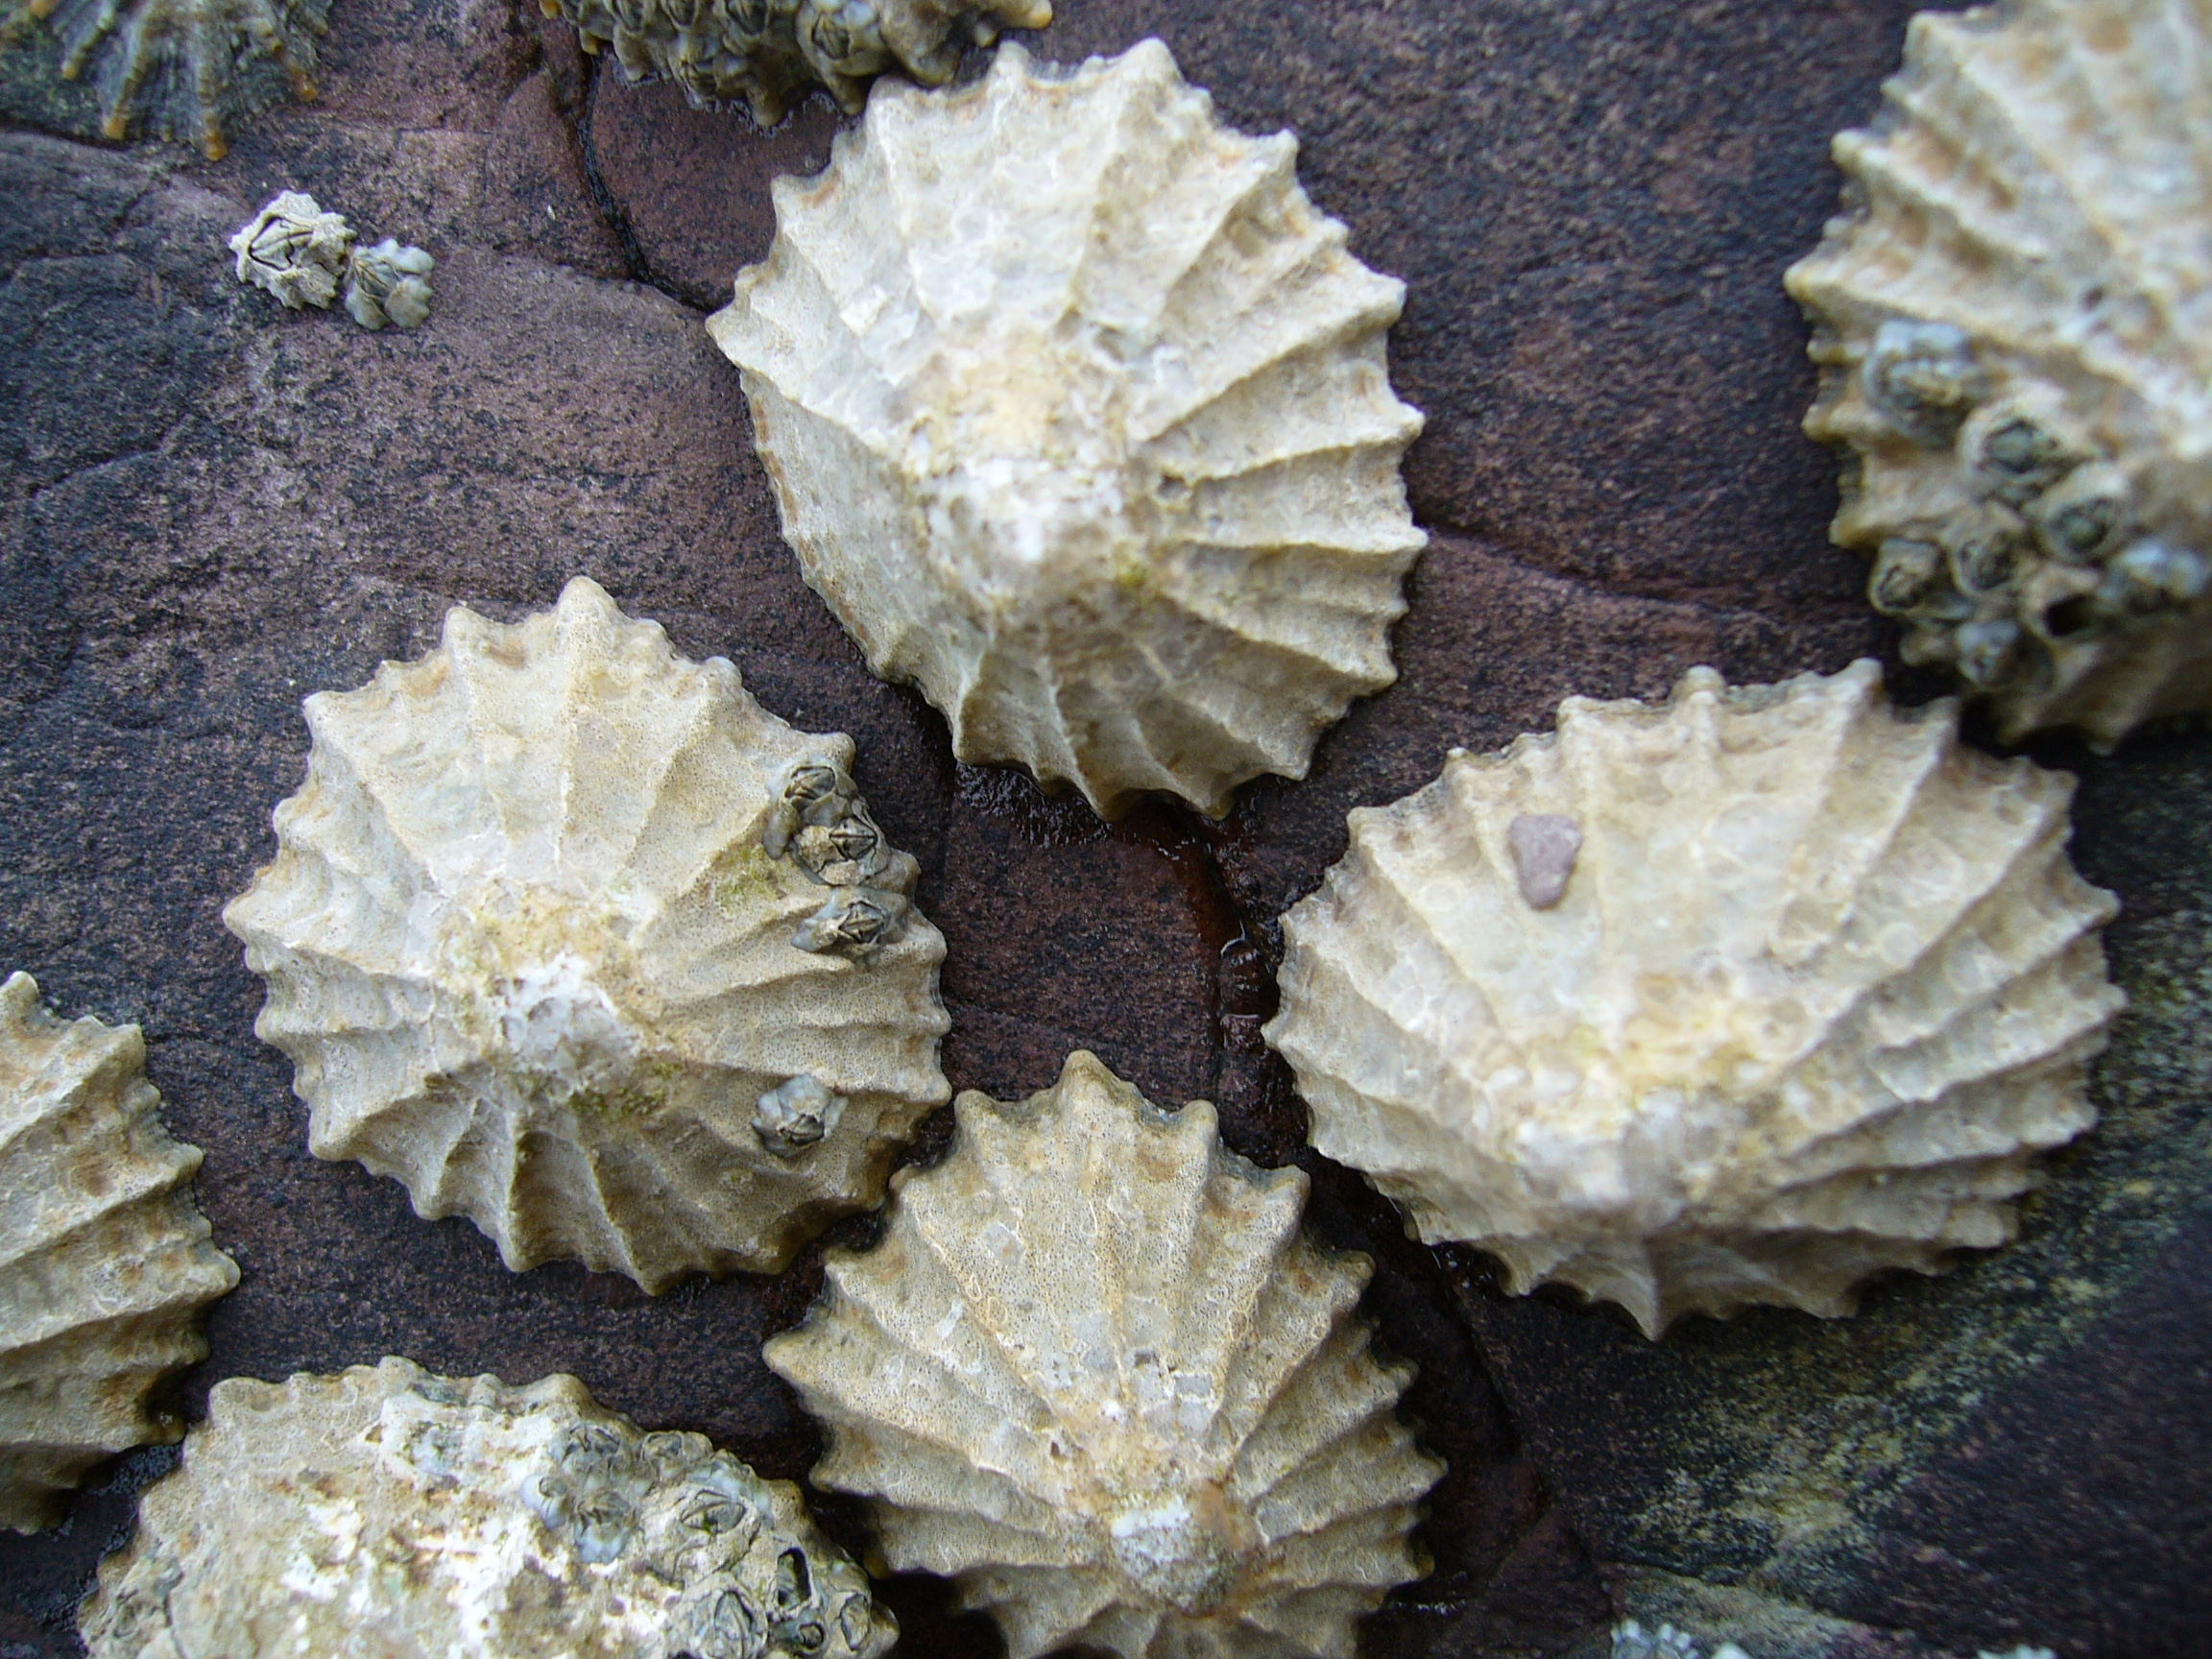
\includegraphics[height=4cm]{imagens/lapas.jpg}
        	\caption{Lapas}
        	\label{fig:lapas}
    	\end{subfigure}%
   	\begin{subfigure}{.5\textwidth}
    	\center
        	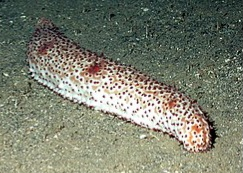
\includegraphics[height=4cm]{imagens/lesma.jpg}
        	\caption{Lesma-do-mar}
       	\label{fig:lesma}
    	\end{subfigure}
    \caption{Gastrópodes}
    	\label{fig:gastropodes}
\end{figure}

\subsection{Crustáceos}
Os crustáceos, membros do subfilo Crustacea, constituem um grupo diversificado de artrópodes marinhos e de água doce. Entre eles, destacam-se os caranguejos (\ref{fig:caranguejo}), lagostas (\ref{fig:lagosta}) e camarões (\ref{fig:camarao}), cada um exibindo características distintas.

Podemos encontrar milhares espécies diferenciadas de caranguejos. Este crustáceo, pode apresentar até dez patas bastante articulas e uma carapaça resistente e achatada que protege o seu corpo.

São conhecidas pelas suas antenas longas e caudas robustas, que ajudam na comunicação e deteção de alimentos. Habitam sobretudo nas regiões rochosas e recifes de coral. Esta espécie alimenta-se sobretudo de peixes e algas.

Os camarões são crustáceos pertencentes à ordem Decapoda. Estes animais podem ser encontrados tanto em água salgada como em água doce, existindo milhares de espécies diferenciadas. Deslocam-se normalmente em cardumes, alimentando-se de microalgas.

\begin{figure}[H]
\center
    \begin{subfigure}{.5\textwidth}
    \center
        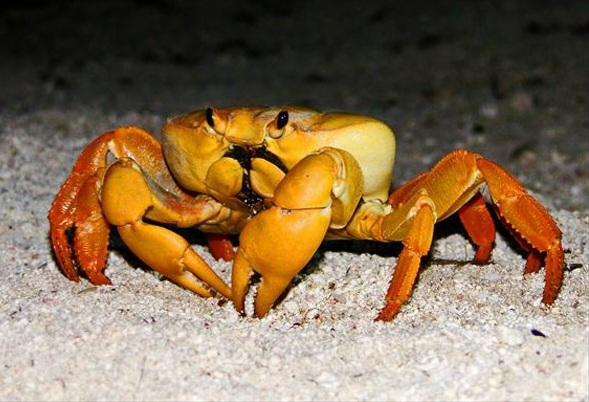
\includegraphics[height=4cm]{imagens/caranguejo.jpg}
        \caption{Caranguejo}
        \label{fig:caranguejo}
    \end{subfigure}%
    \hfill
    \begin{subfigure}{.5\textwidth}
    \center
        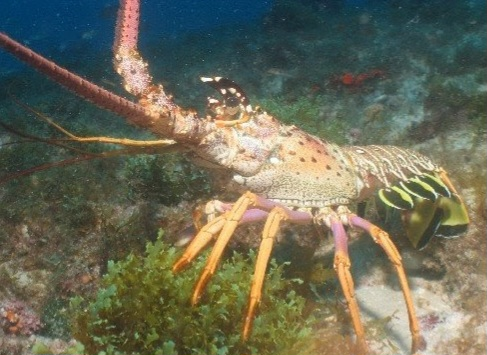
\includegraphics[height=4cm]{imagens/lagosta.jpg}
        \caption{Lagosta}
        \label{fig:lagosta}
    \end{subfigure}%
    \hfill
    \begin{subfigure}{.5\textwidth}
    \center    
        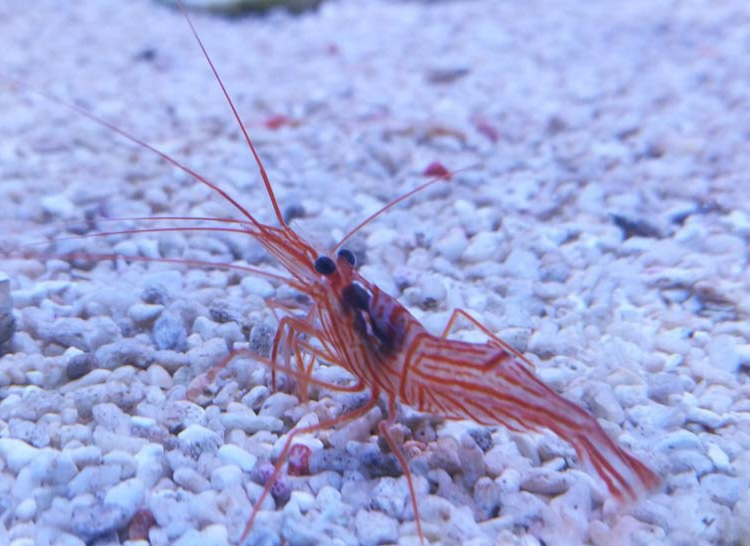
\includegraphics[height=4cm]{imagens/camarao.jpg}
        \caption{Camarão}
        \label{fig:camarao}
    \end{subfigure}
    \caption{Crustáceos}
    \label{fig:crustaceos}
\end{figure}

\subsection{Equinodermos}
Os equino dermos, um grupo exclusivamente marinho, compõem u  filo que inclui organismos como estrelas-do-mar e ouriços-do-mar.

As estrelas-do-mar (\ref{fig:estrela}), pertencentes à classe Asteroidea, apresentam uma simetria radial com braços que irradiam de um centro. Possuem um esqueleto calcificado composto por placas dérmicas.

Já os ouriços-do-mar (\ref{fig:ourico}), representantes da classe Echinoidea, possuem corpos esféricos e cobertos por espinhos.

\begin{figure}[H]
\center
    	\begin{subfigure}{.5\textwidth}
    	\center
        	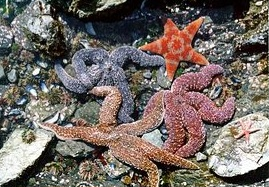
\includegraphics[height=4cm]{imagens/estrela.jpg}
        	\caption{Estrela-do-mar}
        	\label{fig:estrela}
    	\end{subfigure}%
   	\begin{subfigure}{.5\textwidth}
    	\center
        	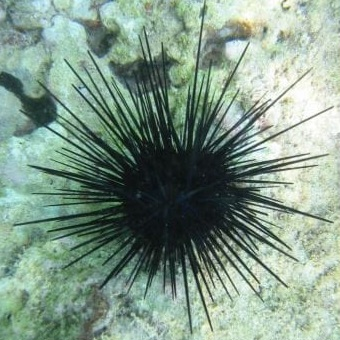
\includegraphics[height=4cm]{imagens/ourico.jpg}
        	\caption{Ouriço-do-mar}
       	\label{fig:ourico}
    	\end{subfigure}
    \caption{Equinodermos}
    	\label{fig:equinodermos}
\end{figure}

\section{Algas}
As algas representam um grupo diversificado de organismos autotróficos fotossintetizantes que desempenham papéis cruciais nos ecossistemas aquáticos.

As algas verdes (\ref{fig:algasverdes}), pertencem a um grupo diversificado de algas que contêm clorofila, o pigmento verde responsável pela fotossíntese. Podem ser unicelulares ou multicelulares.

As algas castanhas (\ref{fig:algascastanhas}), predominantes do filo Phaeophyta, incluem algumas das algas de maior porte, como as \textit{kelps}. São encontradas em águas mais frias.

As algas vermelhas (\ref{fig:algasvermelhas}), podem ser encontradas em profundidades variadas, elas contêm pigmentos, como a ficobilina, que lhes dá uma coloração avermelhada.	


\begin{figure}[H]
\center
    \begin{subfigure}{.5\textwidth}
    \center
        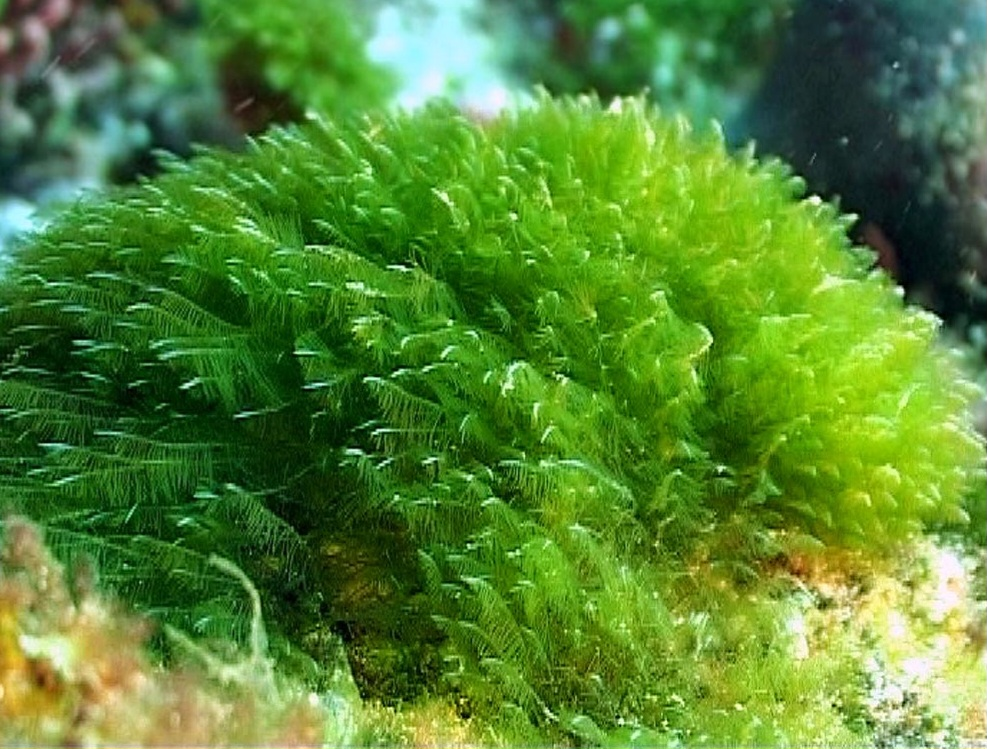
\includegraphics[height=4cm]{imagens/algasverdes.jpg}
        \caption{Algas Verdes}
        \label{fig:algasverdes}
    \end{subfigure}%
    \hfill
    \begin{subfigure}{.5\textwidth}
    \center
        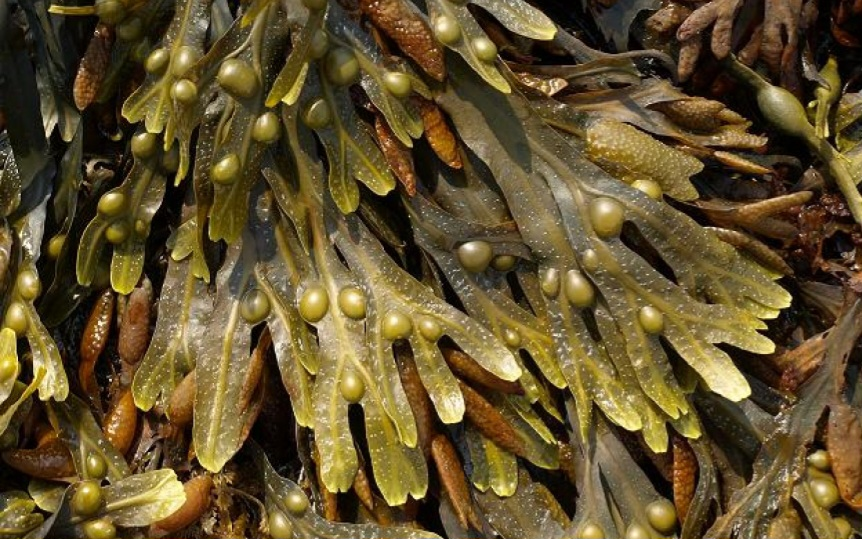
\includegraphics[height=4cm]{imagens/algascastanhas.jpg}
        \caption{Algas Castanhas}
        \label{fig:algascastanhas}
    \end{subfigure}%
    \hfill
    \begin{subfigure}{.5\textwidth}
    \center    
        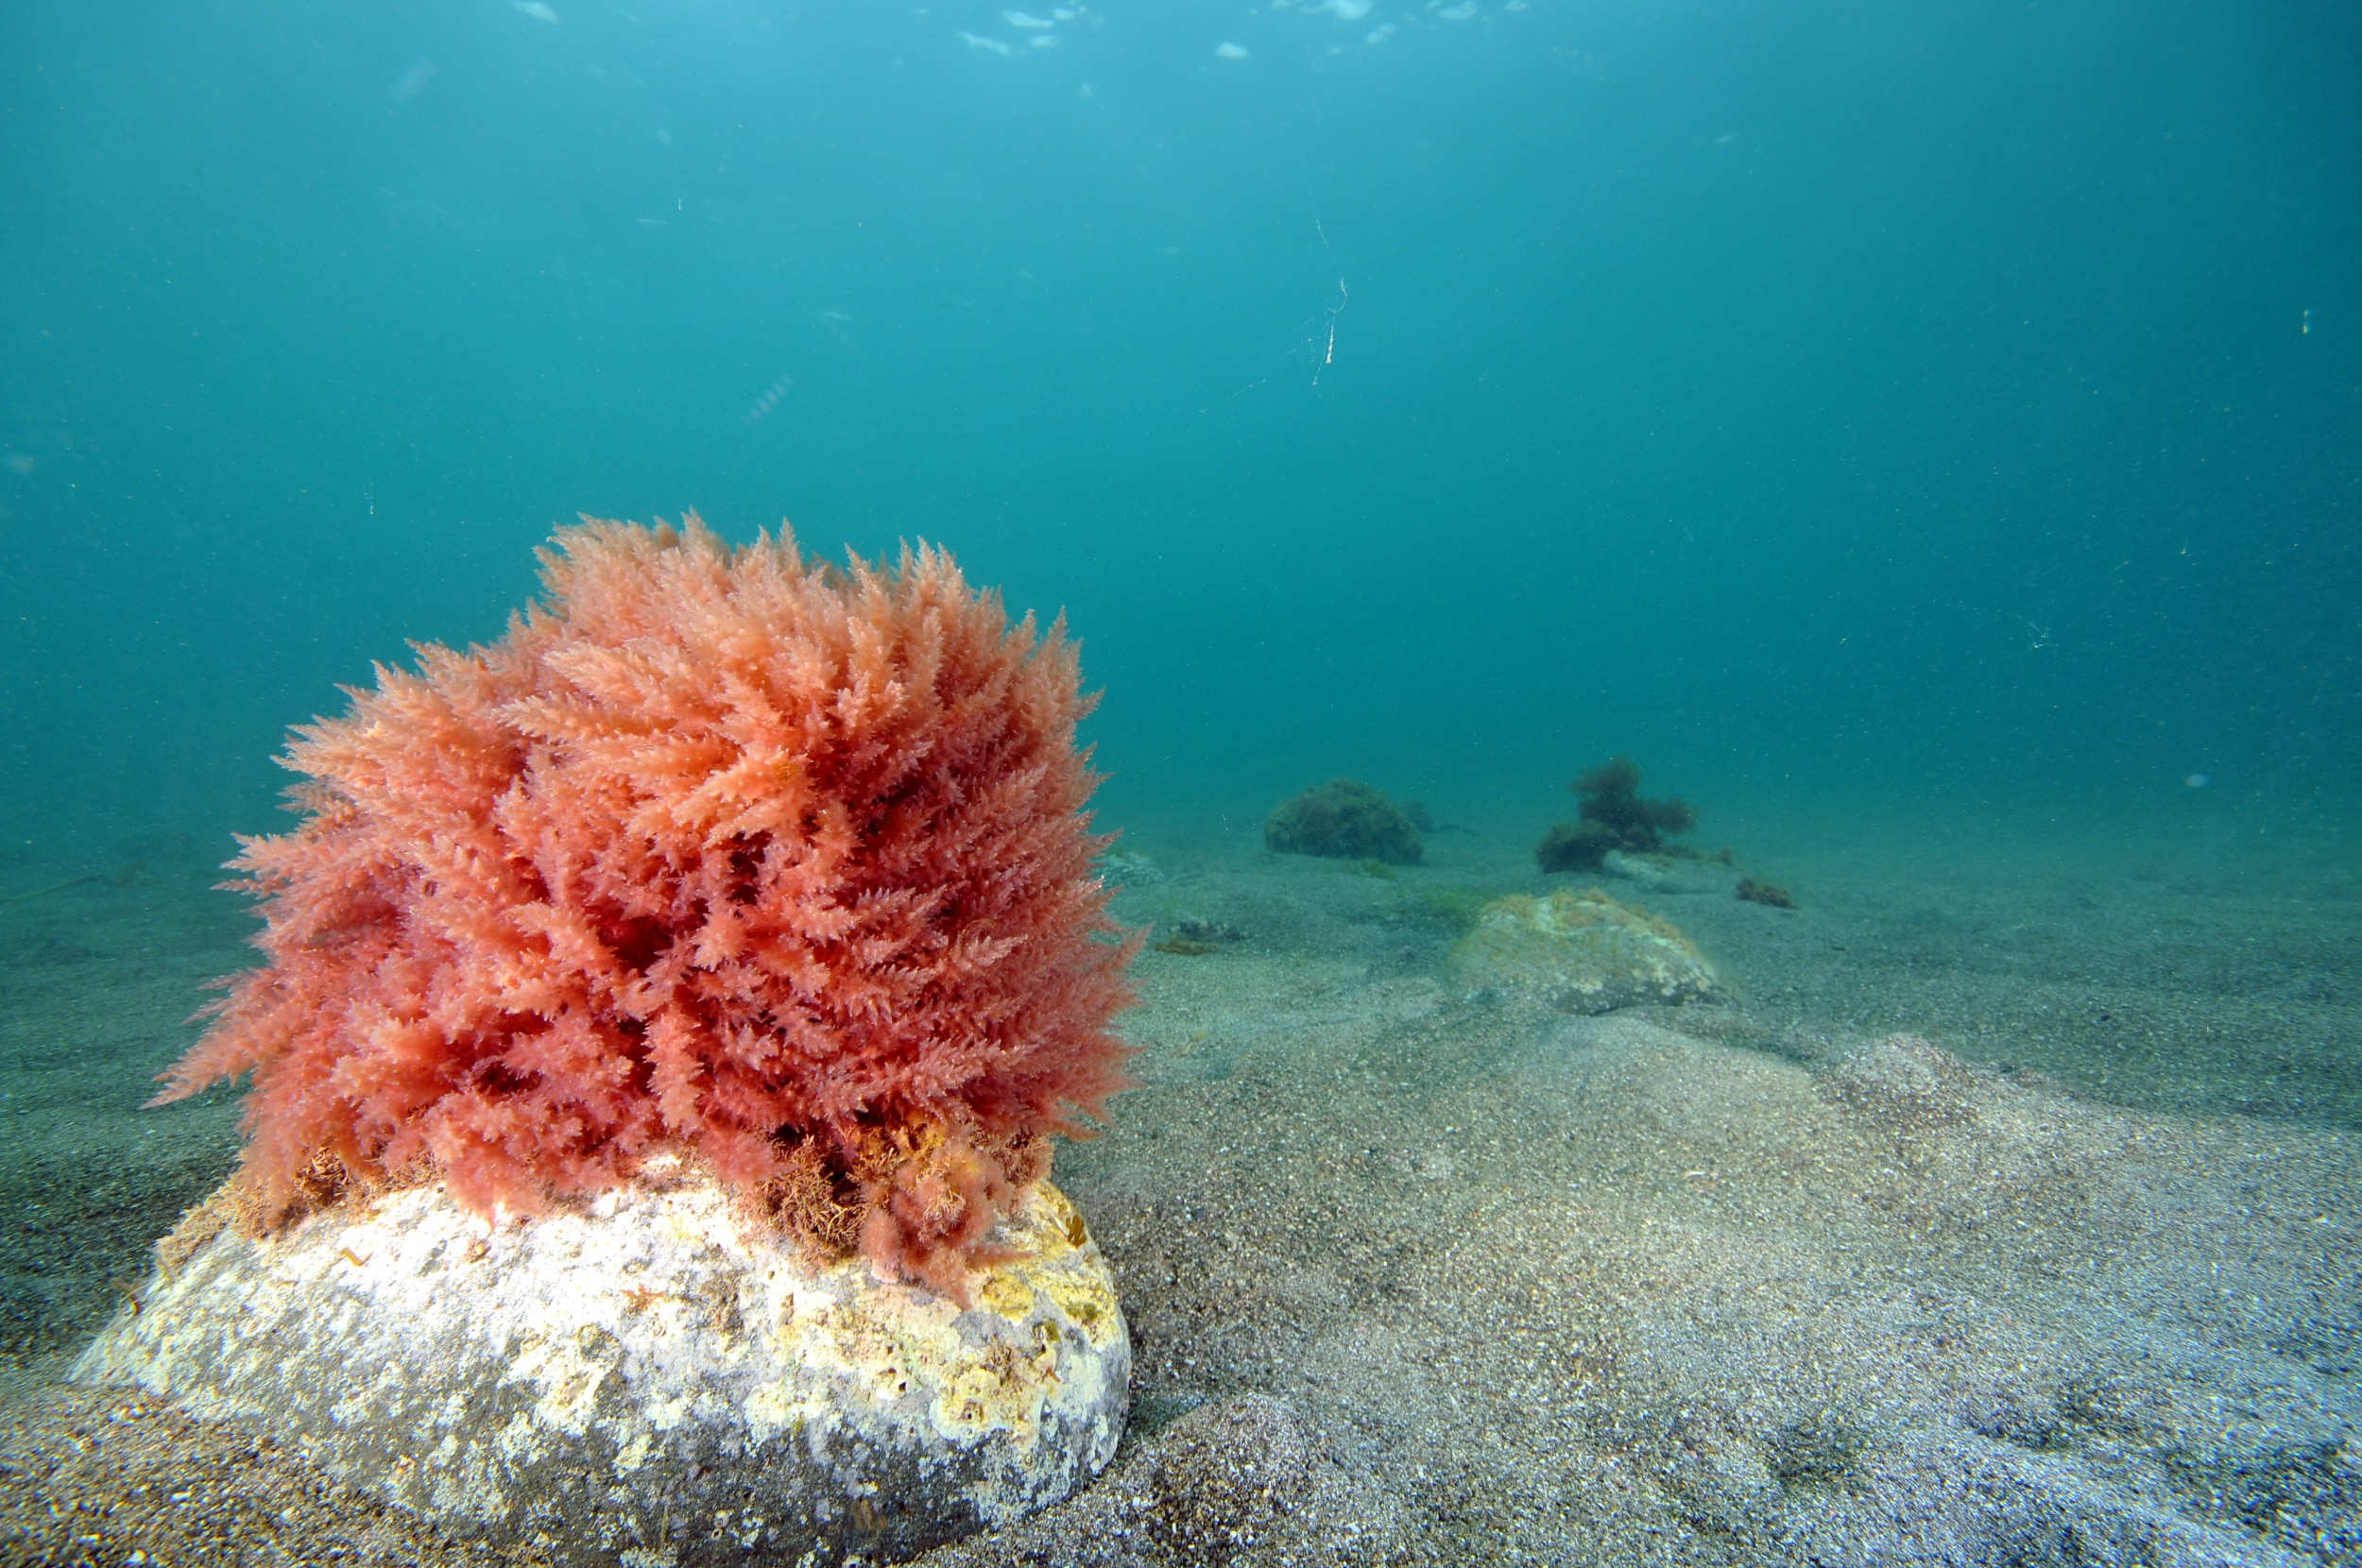
\includegraphics[height=4cm]{imagens/algasvermelhas.jpg}
        \caption{Algas Vermelhas}
        \label{fig:algasvermelhas}
    \end{subfigure}
    \caption{Algas}
    \label{fig:algas}
\end{figure}

\section{Relações Ecológicas}
As relações ecológicas, são essenciais para a sobrevivência e evolução das espécies marinhas, abrangem desde a intensa competição por recursos limitados até às formas de cooperação e dependência.
\subsection{Relações Intraespecíficas}
\subsubsection{Competição por recursos}
Nos ambientes marinhos existe uma busca incessante por recursos escassos. Seja disputando território, alimento ou parceiros reprodutivos, as criaturas marinhas  desenvolveram estratégias para garantir a sua sobrevivência e sucesso reprodutivo.
\\
\\
\begin{tabular}{|c|c|c|} \hline
     Espécie Marinha & Recurso Disputado  & Estratégias de Competição  \\ \hline
    \makecell{Leão-Marinho \\(\textit{Zalphus californianous})} & Espaço na praia & \makecell{Disputas territoriais e \\vocalizações intimidadoras} \\ \hline
    \makecell{Caranguejo-Ermita \\(\textit{Paguroidea})} & \makecell{Conchas \\Disponíveis} & \makecell{Competição por conchas\\ adequadas ao seu tamanho} \\ \hline
    \makecell{Golfinho Nariz-de-Garrafa \\(\textit{Tursiops truncatus})} & Alimento & \makecell{Estratégias de caça \\cooperativa em cardumes} \\ \hline
\end{tabular}
\\
\\
\subsubsection{Comportamento Reprodutivo}
O comportamento reprodutivo na vida marinha é bastante diversificado, desde as danças de acasalamento até comportamentos parentais dedicados, cada espécie desenvolveu estratégias únicas para garantir a continuação da sua linhagem.
\begin{enumerate}
	\item \textbf{Peixe-Palhaço (\textit{Amphiprionidae})}
	O corte nupcial envolve danças coordenadas entre o macho e a fêmea, enquanto a fêmea escolhe um parceiro com base na saúde da anémona onde vivem. O macho torna-se responsável pelos ovos após a desova.
	\item \textbf{Cavalos-Marinhos(\textit{Hippocampus})}
	Em muitas espécies de cavalos-marinhos, é o macho que fica grávido, recebendo os ovos numa bolsa incubadora. Durante o parto, ele contrai a bolsa e libera as crias já formadas.
	\item \textbf{Lula-de-Humboldt (\textit{Dosidicus gigas})}
	As lulas-de-Humboldt formam agregações para acasalamento. Os machos competem para fertilizar os ovos das fêmeas e o acasalamento geralmente ocorre em águas mais profundas.
	\item \textbf{Tartaruga-Marinha (Cheloniidae)}
	As tartarugas-marinhas retornam às praias de nidificação onde nasceram para pôr ovos. A fêmea faz escavações na areia para enterrar os ovos.
	\item \textbf{Estrela-do-Mar (\textit{Asteroidea})}
	Algumas estrelas-do-mar têm a capacidade de se regenerar a partir de partes do corppo, incluindo órgãos reprodutivos. Isso permite que uma estrela-do-mar regenere e crie mais de si mesma.
\end{enumerate}	

\subsection{Relações Interespecíficas}
\subsubsection{Predação e Alimentação}
As interações predatórias são fundamentais nos ecossistemas marinhos, onde várias espécies dependem da predação para alimentação. Isto inclui cadeias alimentares complexas e adaptações evolutivas para caça e defesa.
\\
\\
\begin{tabular}{|c|c|c|} \hline
    Espécie Marinha & Presa & Estratégias de Caça \\ \hline
    \makecell{Tubarão-martelo \\(\textit{Sphyrnidae})} & \makecell{Raias e \\Peixes} & \makecell{Utiliza a forma da cabeça para \\aumentar a eficácia ao capturar \\presas no fundo do oceano.} \\ \hline
    \makecell{Caranguejo Boxeador \\(\textit{Lybia tessellata})} & \makecell{Corais e \\Anémonas} & \makecell{Utiliza as garras para colher \\pedaços de corais e anémonas \\para se defender e alimentar.} \\ \hline
    \makecell{Lula Colossal \\(\textit{Mesonychoteuthis hamiltoni})} & \makecell{Peixes e \\Cefalópodes} & \makecell{Utiliza os tentáculos extensos \\para capturar presas em grandes \\profundidades.} \\ \hline
    \makecell{Tubarão-Branco \\(\textit{Carcharodon carcharias})} & \makecell{Focas e \\Pinguins} & \makecell{Ataques de surpresa nas áreas \\de reprodução e descanço, \\utilizando a emboscada para \\capturar presas menos ágeis.} \\ \hline
\end{tabular}
\\
\\
\subsubsection{Simbiose}
As relações simbióticas são interações íntimas entre diferentes espécies. A simbiose é dividida em Mutualismo, Comensalismo e Parasitismo.
\\
\\
\begin{tabular}{|c|c|c|} \hline
    Espécie A & Espécie B & Tipo de Simbiose \\ \hline
    \makecell{Peixe-Limpador \\(\textit{Labroides spp.})} & \makecell{Tubarões e \\outros grandes \\peixes} & \makecell{Mutualismo. Remove parasitas \\e detritos dos dentes e das \\branquias de peixes maiores, \\obtendo alimento em troca.} \\ \hline
    \makecell{Cracas \\(\textit{Cirripedia})} & \makecell{Baleias e \\Tartarugas} & \makecell{Comensalismo. As Cracas \\fixam-se externamente ao \\casco de baleias e 	\\tartarugas, obtendo \\transporte e alimentação \\filtrando partículas da água.} \\ \hline
    \makecell{Isópode \\(\textit{Cymothoa exigua})} & Peixes & \makecell{Parasitismo. O isópode \\fixa-se à língua de certos \\peixes, substituindo-a e \\ alimentado-se do sangue do peixe} \\ \hline
\end{tabular}


\chapter{Biodiversidade e Ecossistemas da vida marinha}
\label{chap.biodiversidade}

\section{Ecossistemas Marinhos}
Um ecossistema é um conjunto de comunidades de seres vivos e não vivos que interagem entre si e o meio onde vivem, influenciados pelos fatores externos como a água, a luz solar e a temperatura. Os ecossistemas marinhos apresentam características únicas resultantes dos fatores físicos que os contêm, como a alta quantidade de sal nas águas, a temperatura e por vezes a quantidade de luz solar disponível.

\subsection{Principais Ecossistemas}
\label{sub.ecossistemas}
Existem inúmeros ecossistemas marinhos, dos quais:
\begin{itemize}
    \item Mar aberto, que não passa dos 150 metros de profundidade e é encontrado numa zona bem iluminada por radiação solar, a zona eufótica, povoada por espécies fotossintéticas e animais mais conhecidos, como as baleias e algumas espécies de alforreca. 
    \item Mar profundo, que começa por volta dos 200 metros, recebe pouca radiação solar e apresenta temperaturas mais baixas, altos níveis de pressão e pobres níveis de vida, o que faz deste ecossistema um ambiente mais desafiante para os seus habitantes que se alimentam principalmente através de detritos que caem de outros ecossistemas mais próximos da superfície. A maioria dos seres vivos encontrados no mar profundo são espécies de polvos, organismos gelatinosos e alguns peixes mais anormais, como o famoso peixe-futebol.
    \item Recife de corais, um ecossistema com grande biodiversidade, conhecido pelas suas grandes estruturas formadas a partir do esqueleto de carbonato de cálcio de certas espécies de corais e outros animais, encontrado em aguas quentes tropicais, oferece habitat a inúmeras espécies de peixes coloridos como os peixe-papagaio, estrelas do mar, diferentes tipos de esponjas e cobras do mar.
    \item Florestas de algas, normalmente encontradas em aguas frias ou temperadas, são zonas marinhas com alta densidade de macro-algas que fornecem alimento e abrigo a gastrópodes, estrelas marinhas e peixes de potenciais predadores como gaivotas, lontras marinha e focas.
    \item Praias arenosas são ecossistemas únicos pois apresentam diferenças periódicas de amplitude das suas marés, o que divide o próprio ecossistema em três faixas: 
    \begin{enumerate}
        \item A zona superior, onde se encontram espécies marinhas adaptadas à vida terrestre como as pulgas da praia, alguns caranguejos e vários insetos.
        \item A intermédia, menos exposta a marés, povoada principalmente por crustáceos e moluscos que apresentam características para combater a perda de água quando chega a maré baixa.
        \item A faixa inferior, onde habitam espécies sem adaptações especiais à vida fora de água como algumas estrelas do mar e diversas espécies de algas
    \end{enumerate}
    \item Manguezal, um ecossistema costeiro de transição, único pelas suas zonas húmidas onde existe um encontro entre águas de rios com a água do mar. Apresenta um solo salino pobre em oxigénio mas muito rico em nutrientes e por isso aloja uma vegetação diversificada de espécies halófitas, espécies terrestres que evoluíram de forma a sobreviver à salinidade do mar através de raízes aéreas por onde absorvem oxigénio, como varias espécies de mangue e de gramíneas.
\end{itemize}

\section{Zonas do mar profundo}
O mar é divido em varias zonas de acordo com a sua profundidade, as zonas do domínio pelágico. A zona mais superficial é a zona Epipelágica que é a única área considerada como parte da zona eufótica e não ultrapassa os 200m de profundidade. Após a zona superficial as características do ambiente começam a mudar drasticamente e por isso são conhecidas como parte do mar profundo:
\\
\begin{tabular}{|c|c|c|c|c|} \hline
    \multicolumn{5}{|c|}{Profundidade} \\ \hline
     & 200m - 1000m  & 1000m - 4000m & 4000m - 6000m& 6000m - \\ \hline
    Zona & Mesopelágica & Batipelágica & Abissopelágioca  & Hadopelágica \\ \hline
\end{tabular}
\\
\\

A zona Mesopelágica também conhecida como \textit{twilight zone}, não recebe luz solar suficiente para que possa ocorrer fotossíntese, a sua temperatura nas regiões mais quentes do globo pode atingir os 20\textordmasculine C e nas regiões mais frias os 4\textordmasculine C e apresenta uma pressão de 102 atmosferas.

Na zona Batipelágica ou zona Batial encontra-se uma temperatura média de 4\textordmasculine C e pressão de 394 atmosferas. Esta região pertence à zona afótica, onde já não se sente a ação direta da luz solar, e por isso os seus organismos habitantes são independentes de seres fotoautotróficos.

A zona Abissópelagica ou zona Abissal representa 42\% dos fundos oceânicos e apresenta uma temperatura média entre os 2 e os 3\textordmasculine C, uma pressão de 750 atmosferas e é constantemente coberta por escuridão.

A zona Hadopelágica ou zona Hadal faz parte da camada mais interior da zona Abissal e apresenta depressões topográficas longas e estreitas chamadas de fossas abissais que são zonas de encontro entre placas tectónicas onde a pressão chega às 1000 atmosferas. Um exemplo de uma fossa abissal é a Fossa das Marianas, o local mais profundo dos oceanos.
\\
\section{Espécies das Profundezas}
Como o mar profundo não oferece um habitat em que animais fotoautotroficos conseguem viver, o ecossistema destas áreas com profundidade elevada e pouco acesso a luz solar depende apenas de organismos que realizam a quimiossíntese para realizar o papel de produtor primários, o que por vezes pode ser insuficiente. Por causa de todos estes aspetos incomuns muitas espécies do mar profundo apresentam características únicas, como falta de olhos e bioluminescência. Infelizmente, é por causa destas características incomuns que se torna difícil estudar os animais destas zonas, pois elas reagem drasticamente com as mudanças de pressão ou temperatura, o que impossibilita a retirada dos organismos das profundezas.

Na zona Mesopelágica existem peixes que apresentam  bexigas natatórias que os ajudam a controlar a sua flutuabilidade enquanto que outros, como o peixe-lanterna (\ref{fig:peixelanterna}), exibem colorações mais escuras e avermelhadas juntamente com órgãos fotóforos, órgãos produtores de luz, que iluminam a parte inferior do seu corpo numa tentativa de se camuflarem com os raios de luz vindo das águas superiores como método de proteção contra predadores como o peixe-olhos-de-barril (\ref{fig:barreleye}), que apresenta olhos tubulares e uma cabeça transparente, o que lhe proporciona a habilidade de observar tudo o que nada por cima dele.
Os peixe-lanterna, assim como muitas outras espécies da zona Mesopelágica, também apresentam comportamentos migratórios durante a noite e viajam até à camada mais superficial do oceano para fugir a predadores e para perseguir as migrações verticais de zooplâcton de que se alimentam.
Peixes da zona Mesopelágica também exibem adaptações à escassez de comida do seu habitat, como olhos mais sensíveis e mandíbulas maiores. Em alguns predadores também se observam iscas bioluminescentes que são utilizadas para atrair a sua presa. Um exemplo de um predador que utiliza esta tática é o tamboril-com-borlas (\ref{fig:tamboril}), uma espécie de tamboril que exibe uma isca com um aspeto semelhante ao de minhocas ou até crustáceos mais pequenos, que juntamente com a sua habilidade de mudar a cor do seu corpo para facilmente se camuflarem com os seus arredores, e assim caçam a sua presa com maior facilidade.
\\
\begin{figure}[H]
\center
    \begin{subfigure}{.5\textwidth}
    \center
        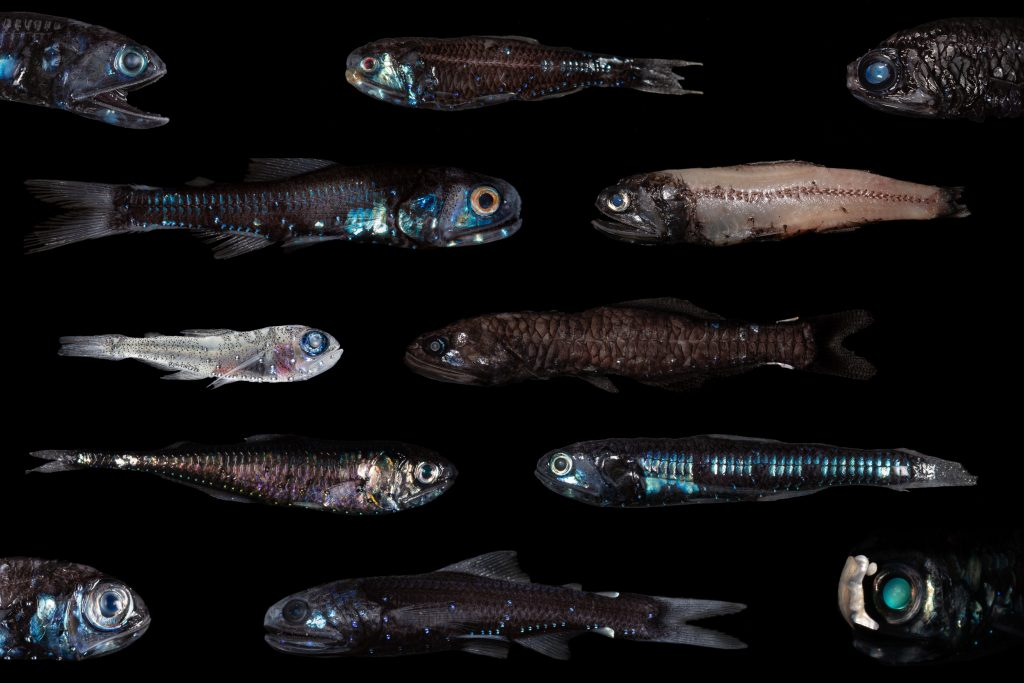
\includegraphics[height=4cm]{imagens/lanternfish.jpeg}
        \caption{peixes da família \textit{Myctophidae}}
        \label{fig:peixelanterna}
    \end{subfigure}%
    \hfill
    \begin{subfigure}{.5\textwidth}
    \center
        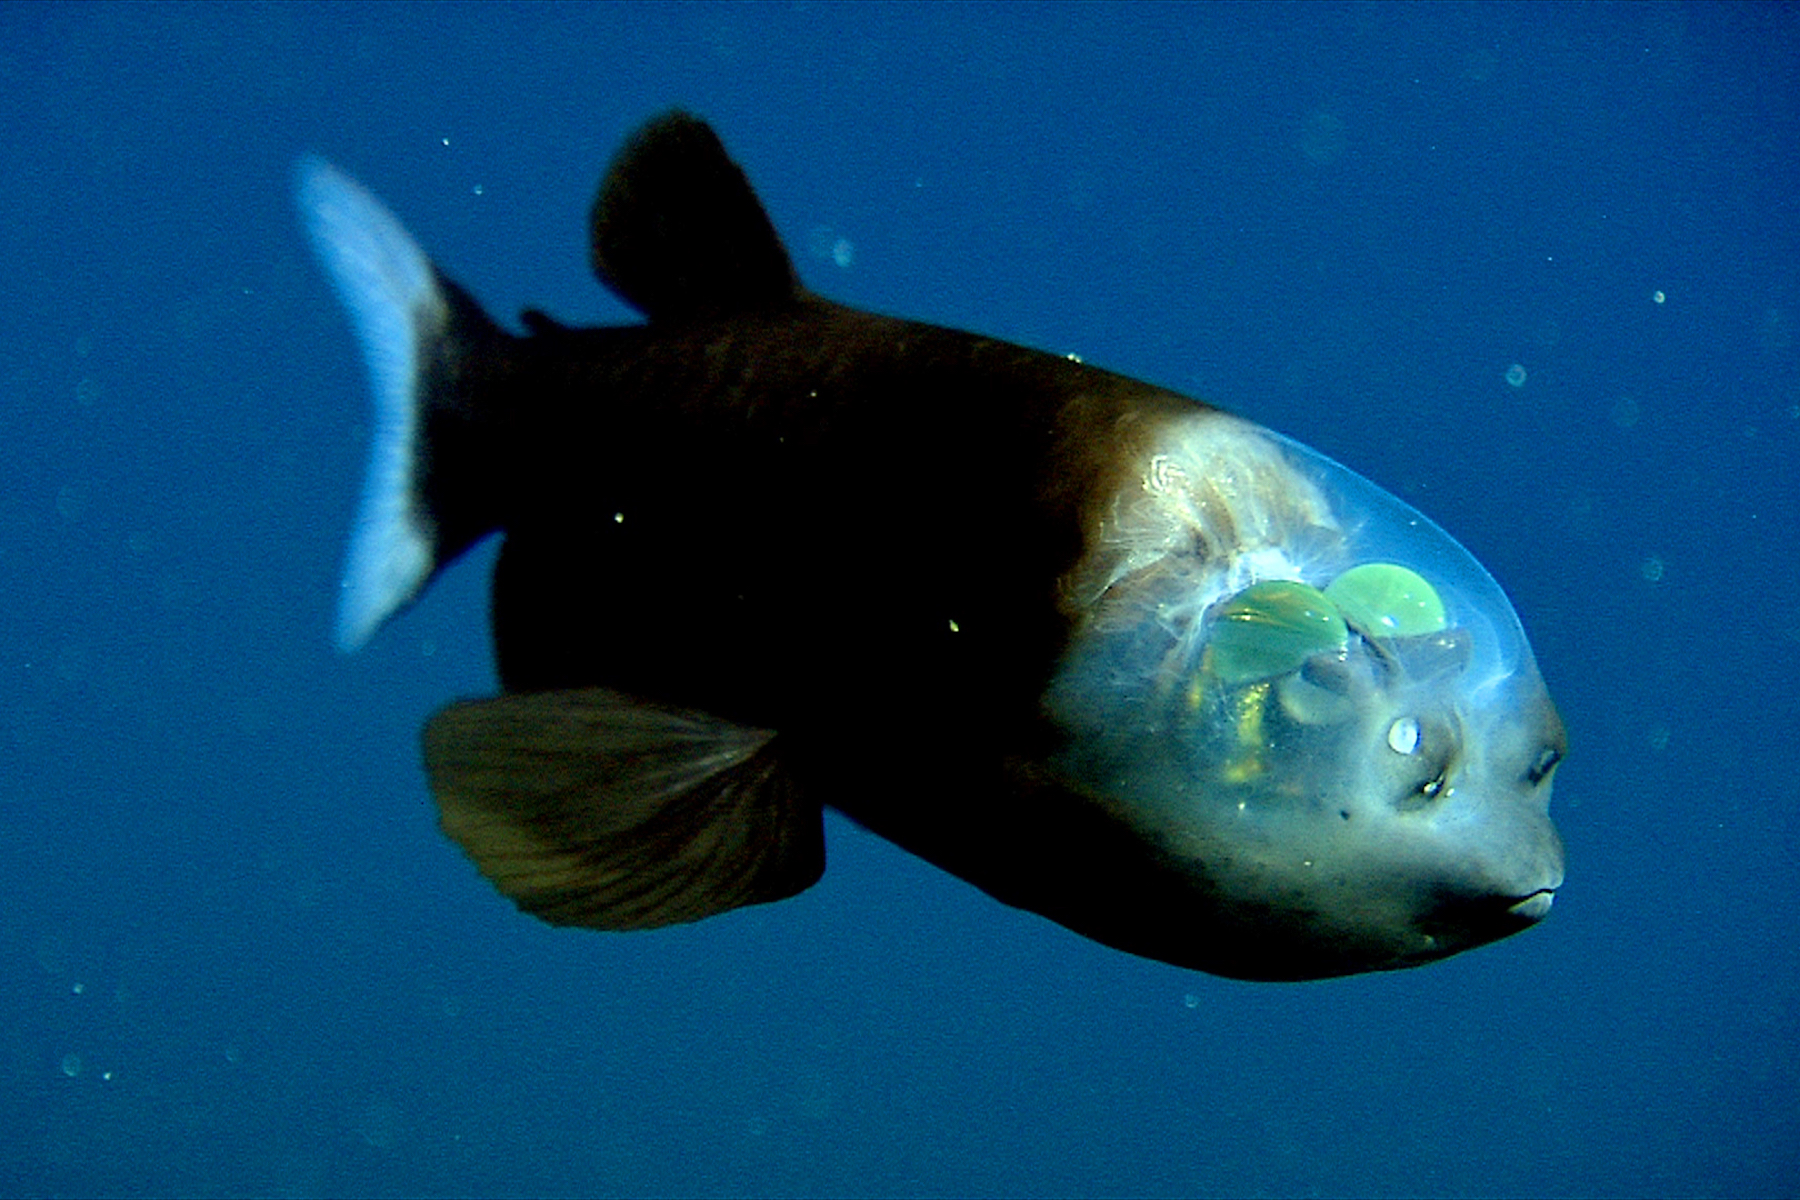
\includegraphics[height=4cm]{imagens/barreleye.jpeg}
        \caption{\textit{Macropinna microstoma}}
        \label{fig:barreleye}
    \end{subfigure}%
    \hfill
    \begin{subfigure}{.5\textwidth}
    \center    
        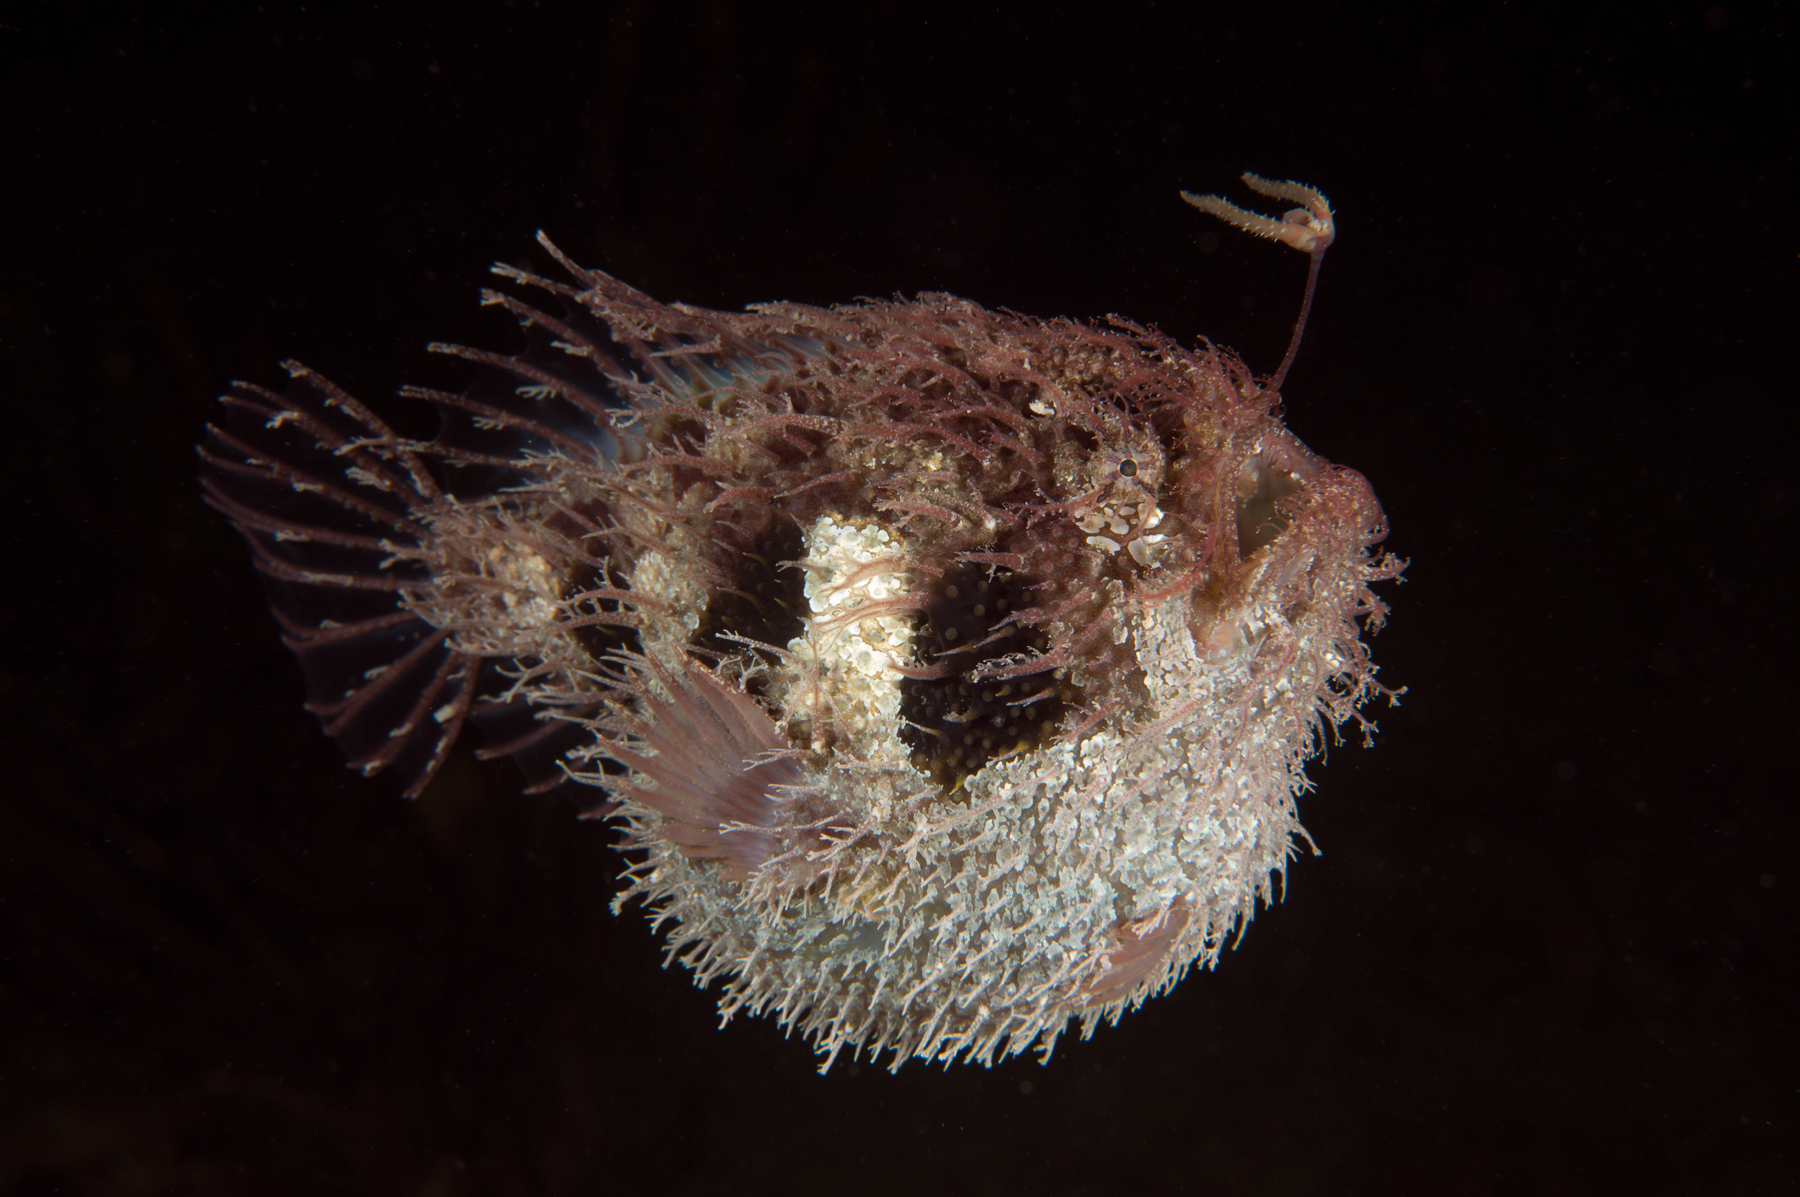
\includegraphics[height=4cm]{imagens/anglerfish.jpg}
        \caption{\textit{Rhycherus filamentosus}}
        \label{fig:tamboril}
    \end{subfigure}
    \caption{Peixes da zona Mesopelágica}
    \label{fig:peixesMeso}
\end{figure}

A zona Batipelágica é um ambiente muito hostil para a vida dos peixes pois alimento é muito escasso, o que resulta na evolução de muitas espécies de modo a terem um metabolismo mais lento de forma a conservar mais energia e necessitar de alimento menos frequentemente. Os peixes desta área apresentam uma dieta bastante variada que utilizam ,juntamente com o seu metabolismo lento, para ficarem escondidos à espera que caia comida de regiões superiores e assim conservam energia que seria gasta à procura de alimento, um bom exemplo de peixe com este estilo de predação é o \textit{bristlemouth} (\ref{fig:bristlemouth}), um peixe minúsculo que apresenta uma mandíbula enorme capaz de apanhar presa maior que o seu próprio corpo. Alguns dos peixes desta profundeza também são predadores ativos, tal como o \textit{telescopefish} (\ref{fig:telescopefish}) que utiliza os seus olhos tubulares, uma forma que lhes garante maior captação de luz mesmo a grandes distâncias, para observar a bioluminescência das suas presas mais facilmente.

\begin{figure}[H]
\center
    \begin{subfigure}{.5\textwidth}
    \center
        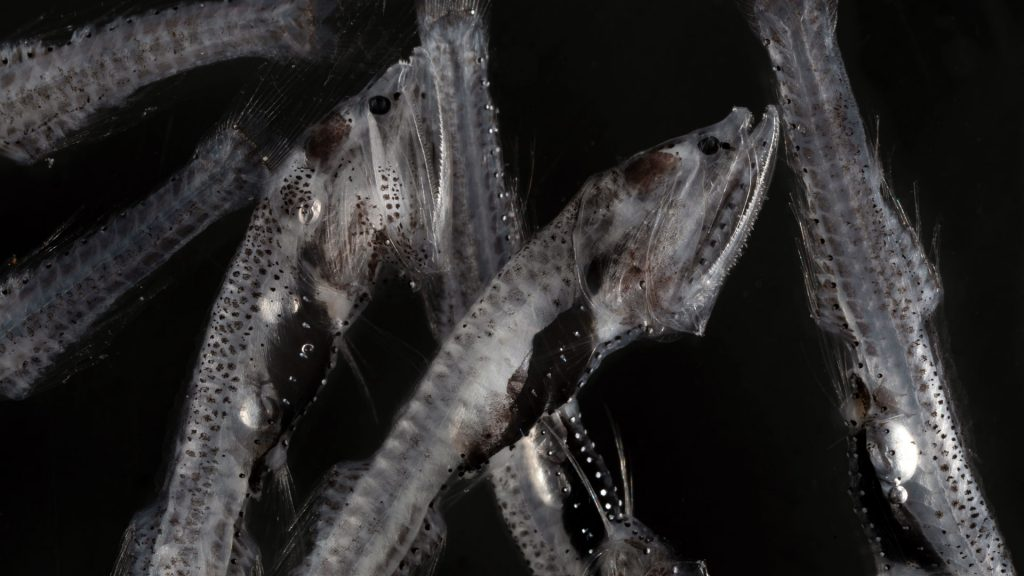
\includegraphics[height=3.5cm]{imagens/Bristlemouth.jpg}
        \caption{ peixes da família \textit{Gonostomatidae }}
        \label{fig:bristlemouth}
    \end{subfigure}%
    \begin{subfigure}{.5\textwidth}
    \center
        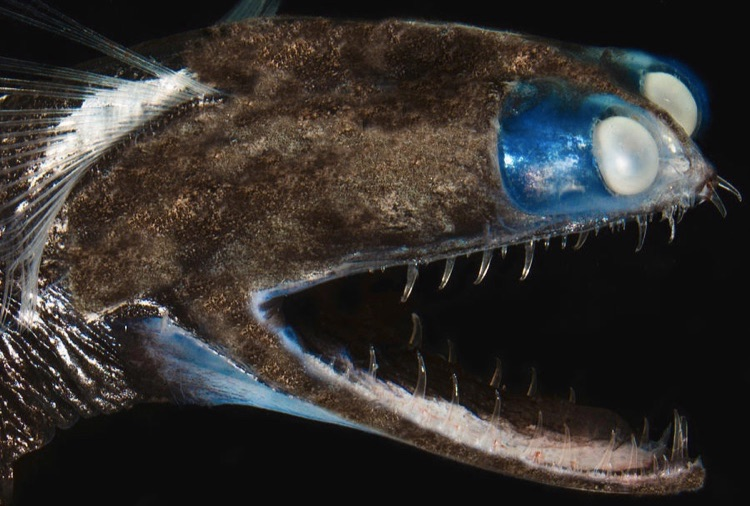
\includegraphics[height=3.5cm]{imagens/telescopefish.jpg}
        \caption{\textit{Giganturidae Giantura}}
        \label{fig:telescopefish}
    \end{subfigure}
    \caption{Peixes da zona Batipelágica}
    \label{fig:peixesBati}
\end{figure}

O oxigénio na zona Abissal é escasso e por isso descer até estas profundezas pode ser fatal para organismos que não apresentam a capacidade de subir até às zonas mais ricas em oxigénio rapidamente. Nesta região são encontrados muitos vestígios de matéria orgânica morta que caiem de zonas superiores, o que faz as águas abissais muito ricas em sais e nutrientes. Estes vestígios que flutuam pelas águas são chamados de neve marinha e servem como alimento para inúmeras espécies naturais da zona Abissopelágica. 
A maioria dos animais que vivem na zona Abissal são animais demersais, ou seja, são organismos que apesar de terem capacidade de natação, permanecem a maior parte da sua vida no fundo do mar e isto acontece pois os seres-vivos abissais dependem dos processos naturais das zonas superiores para sobreviver, e esperam até à queda dos corpos dos animais mortos vindos das zonas acima para se alimentarem.
O polvo-dumbo (\ref{fig:polvodumbo}) é o polvo que vive mais profundamente e é um exemplo de um organismo demersal, ele utiliza as barbatanas localizadas no topo da sua cabeça para "pairar"  sobre o fundo do mar em busca de comida e apesar de ser um polvo, evoluiu de modo não ter um saco de tinta para melhor combater as altas pressões da zona Abissal.

Um peixe demersal desta região é o peixe-tripé (\ref{fig:peixetripe}) que utiliza as barbatanas de osso saliente, localizadas na parte inferior do seu corpo, para se apoiar e posicionar contra-corrente enquanto utiliza as suas "antenas" para sentir quando as suas presas se aproximam. Estas antenas comunicam com as barbatanas frontais e assim que sentem alimento as barbatanas empurram a presa para dentro da boca do peixe.

\begin{figure}[H]
\center
    \begin{subfigure}{.5\textwidth}
    \center
        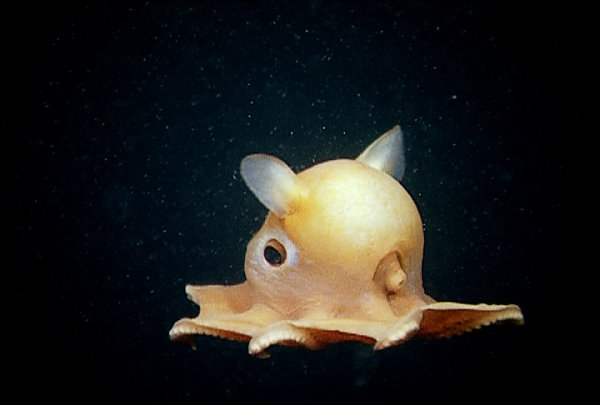
\includegraphics[height=4cm]{imagens/polvodumbo.jpg}
        \caption{polvo do género \textit{Grimpoteuthis}}
        \label{fig:polvodumbo}
    \end{subfigure}%
    \begin{subfigure}{.5\textwidth}
    \center
        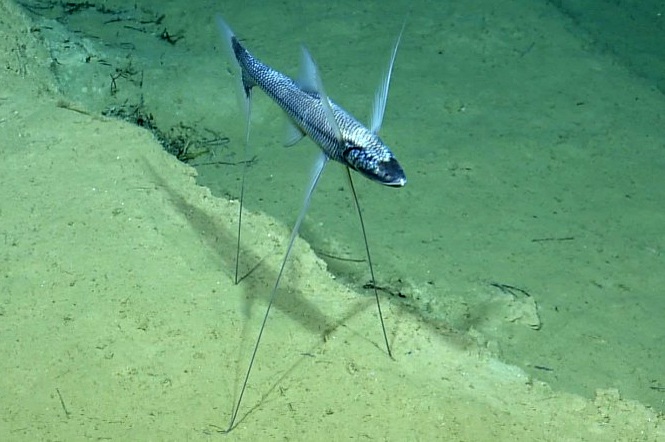
\includegraphics[height=4cm]{imagens/tripodfish.jpg}
        \caption{\textit{Bathypterois grallator}}
        \label{fig:peixetripe}
    \end{subfigure}
    \caption{Organismos da zona Abissal}
    \label{fig:peixesAbiss}
\end{figure}

No mar profundo é muito comum observar que com o aumento da profundidade vem um aumento da massa corporal dos seres-vivos, o que acontece pois uma menor razão de área por volume significa uma maior capacidade de conservação de energia com menos perdas. Este fenómeno é denominado de Gigantismo Abissal e é comum nas áreas mais profundas do oceano por causa da escassez de alimento.

As condições extremas da zona Hadal fazem dela uma área muito difícil de explorar e por isso conhecem-se poucas espécies de lá provenientes. Uma das espécies encontradas foi o peixe-caracol hadal (\ref{fig:snailfish}) cujo corpo contem uma gosma gelatinosa debaixo da pele que os ajuda a melhor controlar a sua flutuabilidade de forma mais simplificada.

O organismo encontrado a maior profundidade até agora foi o \textit{Hirondellea gigas} (\ref{fig:amphipod}), uma espécie de anfípode detritívoro que consume qualquer coisa que caia até ao fundo do oceano, reciclando nutrientes dos materiais mais difíceis de digerir, foram até encontrados micróbios no seu intestino capazes de digerir madeira.

\begin{figure}[H]
\center
    \begin{subfigure}{.5\textwidth}
    \center
        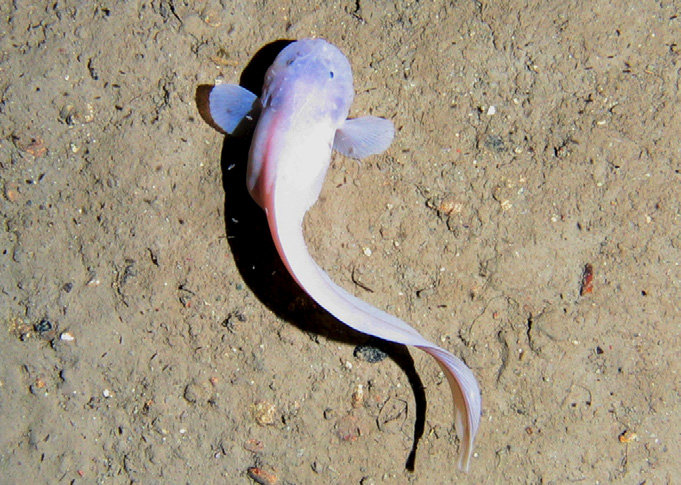
\includegraphics[height=4cm]{imagens/snailfish.jpg}
        \caption{\textit{Pseudoliparis amblystomopsis}}
        \label{fig:snailfish}
    \end{subfigure}%
    \begin{subfigure}{.5\textwidth}
    \center
        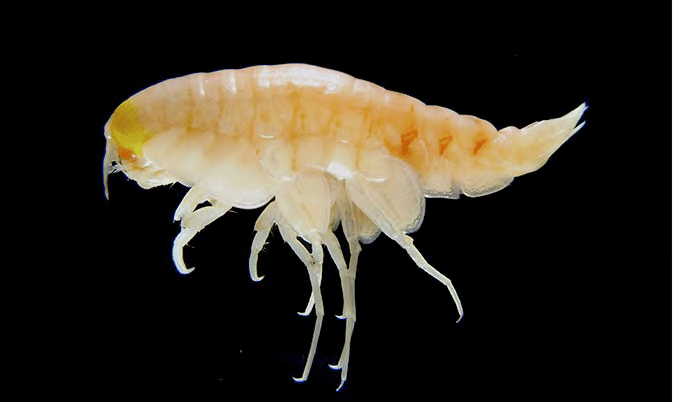
\includegraphics[height=4cm]{imagens/amphipod.png}
        \caption{\textit{Hirondellea gigas}}
        \label{fig:amphipod}
    \end{subfigure}
    \caption{Organismos da zona Hadal}
    \label{fig:peixesHadal}
\end{figure}


\chapter{Impactos Ambientais na Vida Marinha}
\label{chap.impactos}

\section{Introdução}
\label{introducao}
Uma das principais ameaças à vida marinha é a ação humana. Tanto ações diretas, através de atividades como a pesca excessiva e poluição das àguas, como também ações indiretas que contribuem para a acidificação e aquecimento das águas que impactam gravemente os ecossistemas marinhos.


\section{Poluição dos Oceanos}
\label{poluicao}
A poluição marinha é resultado de derrames no mar de produtos químicos, resíduos de atividades agrícolas, industriais ou residências, que podem ser ingeridos por microrganismos ou pequenos animais e assim entram nas cadeias alimentares, podendo contaminar inteiros ecossistemas. 

Uma outra causa de poluição marinha são os derrames de petróleo por navios em alto-mar, que podem ter efeitos devastadores para os ecossistemas marinhos. O petróleo forma uma espécie de barreira à superfície do oceano que impede a penetração da luz, impedindo imensas espécies de realizar fotossíntese, o que consequentemente, afeta toda a cadeia alimentar. O petróleo também é tóxico para animais marinhos que o possam ingerir, como peixes e tartarugas e destrói o pelo de mamíferos marinhos que possam entrar em contacto com o óleo. 


\begin{figure}[H]
    \center
    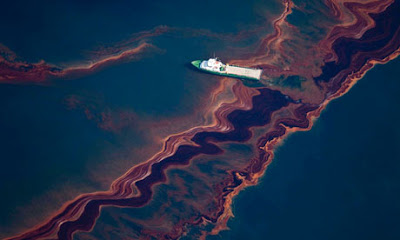
\includegraphics[height=4cm]{imagens/oil-spill.jpg}
    \caption{Derrame de petróleo em alto-mar}
    \label{fig:Derrame_petroleo}
\end{figure}


\section{Acidificação Oceânica}
\label{acidificacao}
As grandes quantidades de $CO_{2}$ libertadas para a atmosfera, não só influenciam os oceanos através do aquecimento global mas também influenciam diretamente as suas águas, que absorvem parte destes gases libertados, o que resulta num aumento do pH da água oceânica. Uma maior acidez das águas traduz-se na malformação de algumas espécies marinhas, principalmente espécies que dependem de carbonato de cálcio para formarem algumas estruturas corporais rígidas, como corais, crustáceos e moluscos que ficam incapazes de gerar uma concha forte suficiente. Uma menor taxa de calcificação afeta todos os aspetos da vida destes organismos, desde a sua reprodução até a sua capacidade de tolerar mudanças na temperatura das águas onde habitam, colocando-os numa situação ainda mais vulnerável face às ameaças do seu habitat.

\section{Impactos do Aquecimento Global}
\label{impactos}
O aquecimento global exerce uma série de impactos na vida marinha, alterando ecossistemas e afetando negativamente várias espécies.

O aumento da temperatura da água dos oceanos está relacionado com o branqueamento dos corais (\ref{fig:branqueamento}). Quando os corais ficam expostos a temperaturas elevadas por períodos prolongados eles expulsam algas simbíoticas que lhes proporcionam cor e nutrientes, o que enfraquece os corais, tornando-os mais suscetíveis a doenças e ameaçando espécies que dependem destes recifes.

\begin{figure}[H]
    \center
        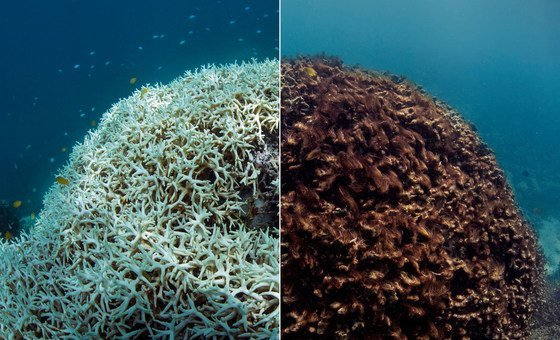
\includegraphics[height=4cm]{imagens/antes_e_depois.jpg}
        \caption{Antes e depois do branqueamento de corais}
        \label{fig:branqueamento}
\end{figure}

O aquecimento global também influencia a distribuição geográfica das espécies marinhas. À medida que as águas aquecem, algumas espécies podem migrar para águas mais frias em busca de ambientes adequados à sua sobrevivência.

Espécies que já estão em risco, como tartarugas marinhas e focas, enfrentam ameaças devido ao aquecimento global. Mudanças no ambiente, como o derretimento do gelo , podem comprometer os habitats essenciais para estas espécies.


\section{Extinções}
\label{extincoes}
Os impactos ambientais na vida marinha têm desencadeado uma onda de extinção preocupante. Diversos fatores têm contribuído para esse cenário alarmante, sendo a poluição dos oceanos uma das principais ameaças. 

A pesca ilegal, não só afeta as espécies que são caçadas, como também trás consequências à cadeia alimentar. Golfinhos, tartarugas, baleias e outras criaturas marinhas são alvos deste comércio ilegal. Como consequência a cadeia alimentar desfaz-se, deixando um rasto de extinção.

O aquecimento global e a acidificação dos oceanos desencadeiam um colapso nos ecossistemas marinhos. Os recifes de coral, que sustentam uma grande variedade de espécies, como foi referido anteriormente no tópico \ref{sec:impactos}, ficam enfraquecidos e mais suscetíveis a doenças por causa do aquecimento e acidificação dos oceanos, prejudicando também as espécies que dependem deles.

A poluição dos mares, proveniente do descarte inadequado de resíduos, ameaça toda a cadeia alimentar marinha. Tartarugas marinhas, baleias e peixes enfrentam diversos perigos, desde a ingestão de plásticos até à contaminação por produtos tóxicos. 

A destruição de habitat também é uma das principais ameaças à biodiversidade marinha, pois muitas espécies marinhas dependem de áreas específicas para reprodução e desova. A destruição destes habitats pode resultar na perda de locais essenciais para o ciclo reprodutivo de várias espécies. A poluição resultante de atividades humanas também contribui para a destruição de ambientes marinhos, pois pode cobrir leitos e sufocar organismos que dependem da luz solar para a sobrevivência, afetando a fauna e a flora locais.





\section{Medidas de Conservação}
\label{medidas}
A conservação da vida marinha é uma tarefa importante para preservar a biodiversidade dos oceanos. Podem ser implementadas várias medidas para acalmar os impactos ambientais na vida marinha:
\begin{enumerate}
\item \textbf{Áreas Marinhas Protegidas:}

Estabelecer áreas marinhas protegidas onde atividades humanas como a pesca e a exploração de recursos são proibidas. Essas áreas forneceriam um refúgio seguro para reprodução, alimentação e crescimento de espécies marinhas.

\item \textbf{Redução da Poluição Marinha:}

Implementar medidas para reduzir a poluição marinha, como o controlo do descarte de resíduos plásticos, produtos químicos e esgoto.
 
\item \textbf{Restauração de Ecossistemas Marinhos:}

Investir em projetos de restauração de ecossistemas marinhos, como por exemplo a recuperação dos recifes de corais.

\item \textbf{Controlo da Acidificação dos Oceanos:}

Reduzir emissões de $CO_{2}$ para controlar a acidificação dos oceanos. Isso envolveria a transição para fontes de energia mais limpas e renováveis, como solar, eólica e hidroelétrica.

\item \textbf{Educação e Sensibilização:}

Promover a educação ambiental e sensibilização pública sobre a importância da vida marinha e os impactos das atividades humanas nos oceanos, que pode levar a mudanças de comportamento e apoio a iniciativas de conservação.


\end{enumerate}

\chapter{Conclusões}
\label{chap.conclusao}
As conclusões tiradas deste trabalho sobre a vida marinha oferecem ao leitor uma visão abrangente e preocupante sobre o estado da mesma:

Começando no \autoref{chap.classificação} que nos permite compreender a classificação da vida marinha, fornecendo uma base para apreciar a diversidade presente nos oceanos, desde os peixes e mamíferos até aos invertebrados, algas e as complexas relações ecológicas que sustentam essas formas de vida. Ao explorar a biodiversidade e os ecossistemas marinhos no \autoref{chap.biodiversidade}, torna-se evidente que esses ambientes são cruciais para a sobrevivência de muitas espécies e a conservação desses ecossistemas é vital não apenas para a vida marinha, mas também para o equilíbrio global. No \autoref{chap.impactos} sobre os impactos ambientais na vida marinha, destaca-se a alarmante realidade das ameaças impostas pela poluição e acidificação dos oceanos, aquecimento global e riscos de extinção que ameaçam a saúde dos ecossistemas marinhos e a sobrevivência de inúmeras espécies.

Portanto, é importante que sejam adotadas medidas rigorosas para reduzir a poluição dos oceanos e promover a conservação dos ecossistemas marinhos. O futuro da vida marinha depende das decisões tomadas hoje, e é responsabilidade de todos nós agir em prol da sustentabilidade e preservação dos ecossistemas marinhos que sustentam a vida no nosso planeta.


\chapter*{Contribuições dos autores}
O elemento \ac{ct} realizou a pesquisa dos conteúdos abordados no \autoref{chap.introducao}, no \autoref{chap.biodiversidade}, nas Secções \ref{introducao}, \ref{poluicao}, \ref{acidificacao} do \autoref{chap.impactos}, assim como a organização dos mesmos, também realizou o Resumo e a Bibliografia.

O elemento \ac{jm} realizou a pesquisa dos conteúdos abordados no \autoref{chap.classificação}, no \autoref{chap.conclusao} nas Secções \ref{impactos}, \ref{extincoes}, \ref{medidas}, assim como a organização dos mesmos.

\vspace{10pt}
\textbf{Percentagem de contribuição de cada autor:}\\

\autores : 50\%, 50\%\\

%%%%%%%%%%%%%%%%%%%%%%%%%%%%%%%%%
\chapter*{Acrónimos}
\begin{acronym}
\acro{ua}[UA]{Universidade de Aveiro}
\acro{leci}[LECI]{Licenciatura em Engenharia de Computadores e Informática}
\acro{glisc}[GLISC]{Grey Literature International Steering Committee}
\acro{ct}[CT]{Carolina Teixeira}
\acro{jm}[JM]{João Martins}
\end{acronym}


%%%%%%%%%%%%%%%%%%%%%%%%%%%%%%%%%
\nocite{*}
\printbibliography

\end{document}